\chapter{Event Selection}
\label{cha:eventsel}

After establishing the signature, datasets, Monte Carlo samples and object selection recipes, one can select the relevant events. Improving the signal to background ratio is the major goal to achieve through this procedure. The motivation behind that, is the large difference in cross sections between the signal and all two muon, two jets processes. The same sign charge requirement is expected to have the biggest impact in that regard. Prior to that, the steps mainly concentrate on reducing \textit{one} dominant background process at a time.

It should also be noted that this analysis was performed ``blindly''. Therefore control regions are used to estimate the agreement before one inspects the final distribution.

\section{Event Cleaning}
\label{sec:evclean}

As a first step, a list of noise filters needs to be applied to the triggered events. Their purpose is to prevent a variety of detector specific effects to be misinterpreted as particles. It is maintained by the JetMET physics object group~\cite{jmepog}. The recommended list~\cite{jmefilters} of noise cleaning filters encompasses the following entries.

\begin{itemize}
\item \textbf{CSC tight beam halo filter} - Uses information of the cathode strip chambers to identify anomalous MET created by the beam halo.
\item \textbf{HBHE noise filter with isolated noise rejection} - Detects isolated noise of instrumental origin. In particular the one from hybrid photodiodes and readout boxes.
\item \textbf{HCAL laser filter} - Picks events where the HCAL laser fired at incorrect times. This leads to numerous entries throughout the entire HCAL.
\item \textbf{ECAL dead cell trigger primitive filter} - Suppresses events where the trigger primitive energy lies above a certain threshold. These mismeasurements are due to the $\sim 1\pct$ of dead ECAL cells.
\item \textbf{Tracking failure filter} - Wards against two issues. Large clusters of entries can lead to less iterations of the tracking algorithm. Displaced primary vertices can also pose problems.
\item \textbf{Bad EE Supercrystal filter} - Two of the $5 \times 5$ crystal regions appear to be provide anomalous information. Removing these events is this filter's task.
\item \textbf{ECAL laser correction filter} - Due to a poor calibration of some ECAL crystals using lasers, they are highly energetic. To prevent a MET mismeasurement, the respective events are removed. 
\item \textbf{Tracking POG filters} - Filters two types of issues. Events with (partially) aborted track reconstruction and events influenced by strip tracker noise.
\end{itemize}

This first stage of the analysis combines event cleaning with the \textbf{electron veto}. The latter is essentially seen as additional noise in regards to selecting muons.

\section{Basic Muon Selection}
\label{sec:basicmuon}

At this stage of the analysis, a first subset of muons is selected. Using the object selection recipe (Sec.~\ref{sec:muonid}) as a basis, the requirements are slightly tightened. Events with less than two muons passing the object identification are rejected immediately.

The \verb+HLT_Mu17_TkMu8+ trigger requires more than $17\,\text{GeV}$ and $8\,\text{GeV}$ transverse momentum for the respective muon. To avoid trigger inefficiencies~\cite{trigeff} in the region close to that cut-off, the following thresholds have been chosen in the analysis. The value for the leading muons is required to be at least $p_{\text{T}} > 20\,\text{GeV}$, while the sub-leading one needs a minimum of $p_{\text{T}} > 15\,\text{GeV}$.

\section{Jet Quality Criteria}
\label{sec:jetqualy}

Since jets cannot be reconstructed as well as muons, their recipe for identification (Sec.~\ref{sec:jetid}) is not altered significantly. Thus they their selection supports, but does not hinder the one for muons.

To satisfy the final state of the signal, the number of jets cannot be lower than two. In addition to that, both the leading and sub-leading jets in terms of transverse momentum, need to pass the $30\,\text{GeV}$ barrier. This is meant to help against clustered tracks or pileup contamination that may be identified as jets. Both the distributions of the number of jets (Fig.~\ref{fig:jetn}) and the leading jet transverse momentum (Fig.~\ref{fig:jetpt1}) show that these requirements mainly suppresses the Drell-Yan background.

\begin{figure}[htb!]
  \centering
  \begin{subfigure}[b]{0.495\textwidth}
    \centering
    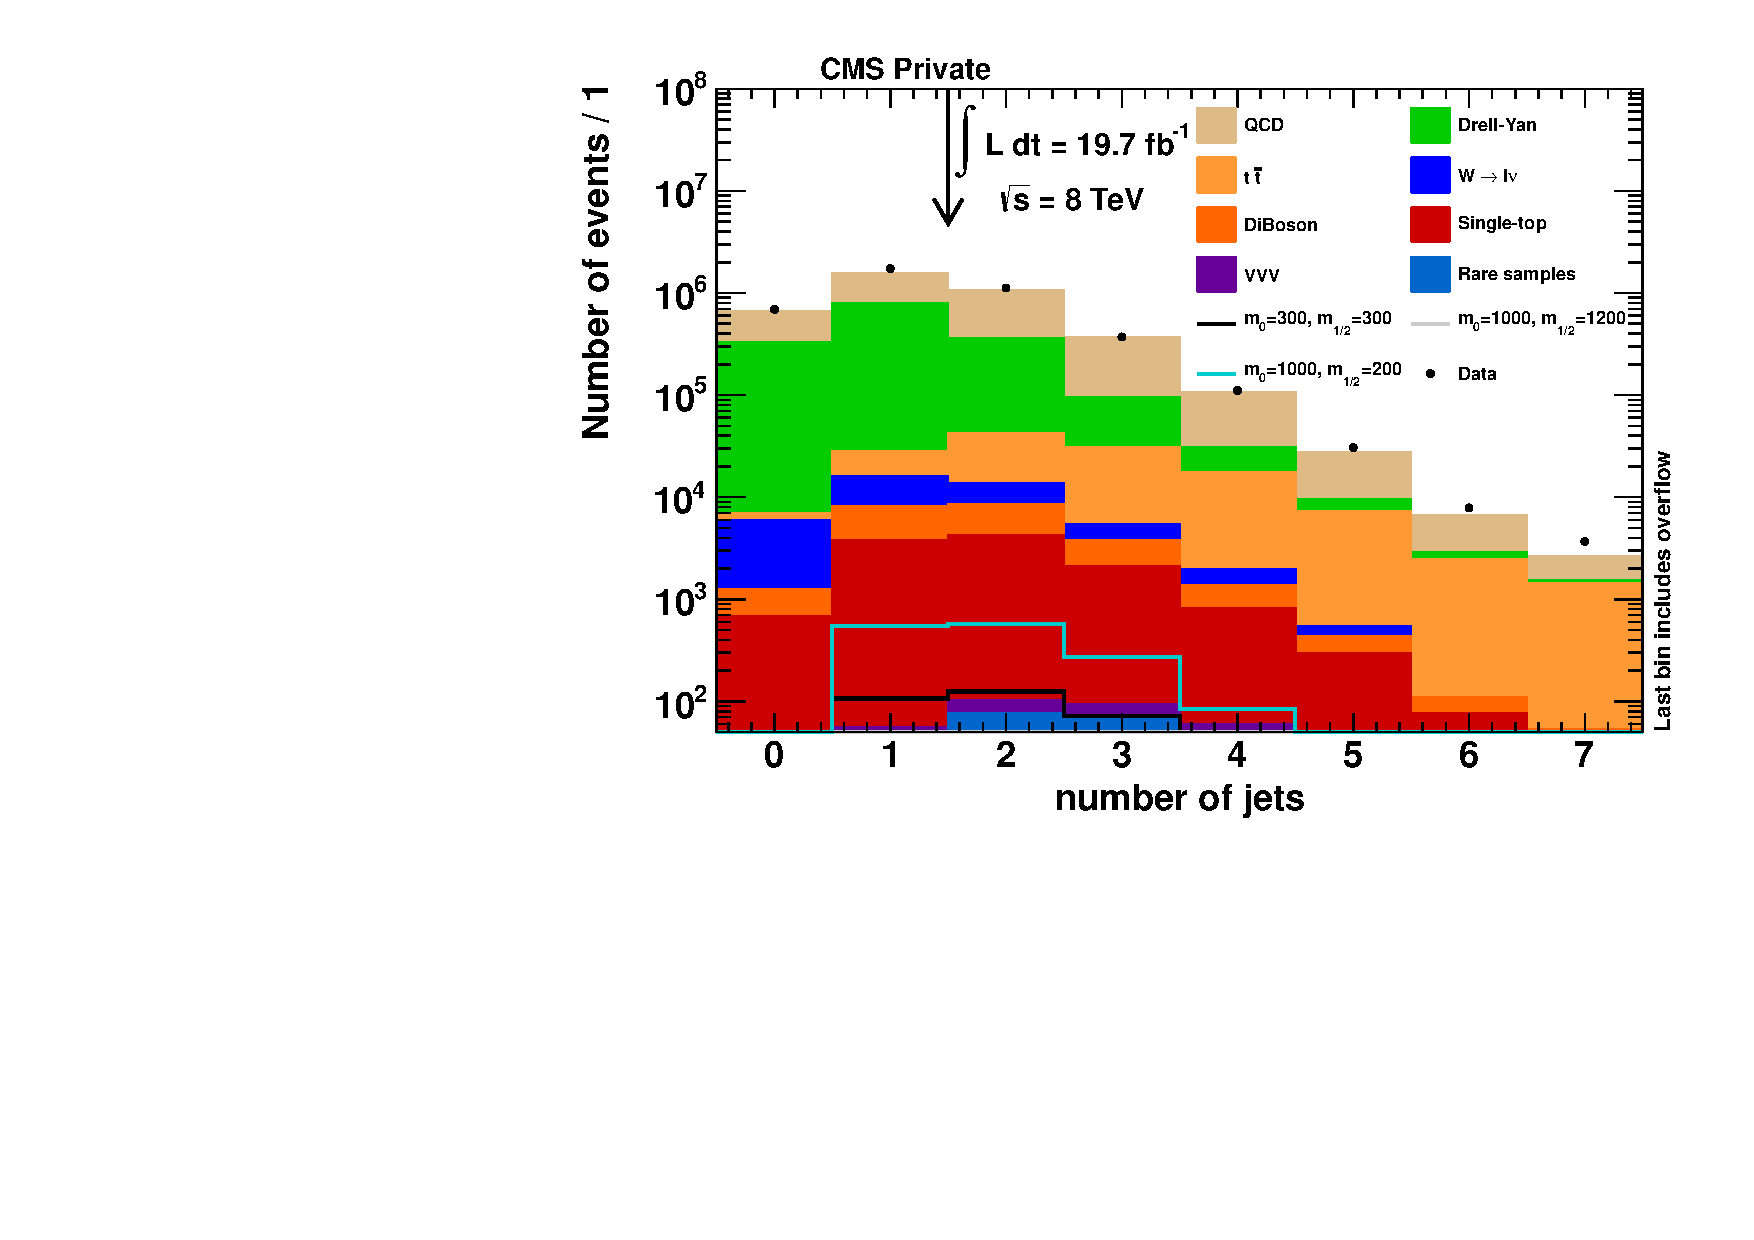
\includegraphics[width=\textwidth]{plots/jet_n.pdf}
    \caption{\label{fig:jetn}}
  \end{subfigure}
  \begin{subfigure}[b]{0.495\textwidth}
    \centering
    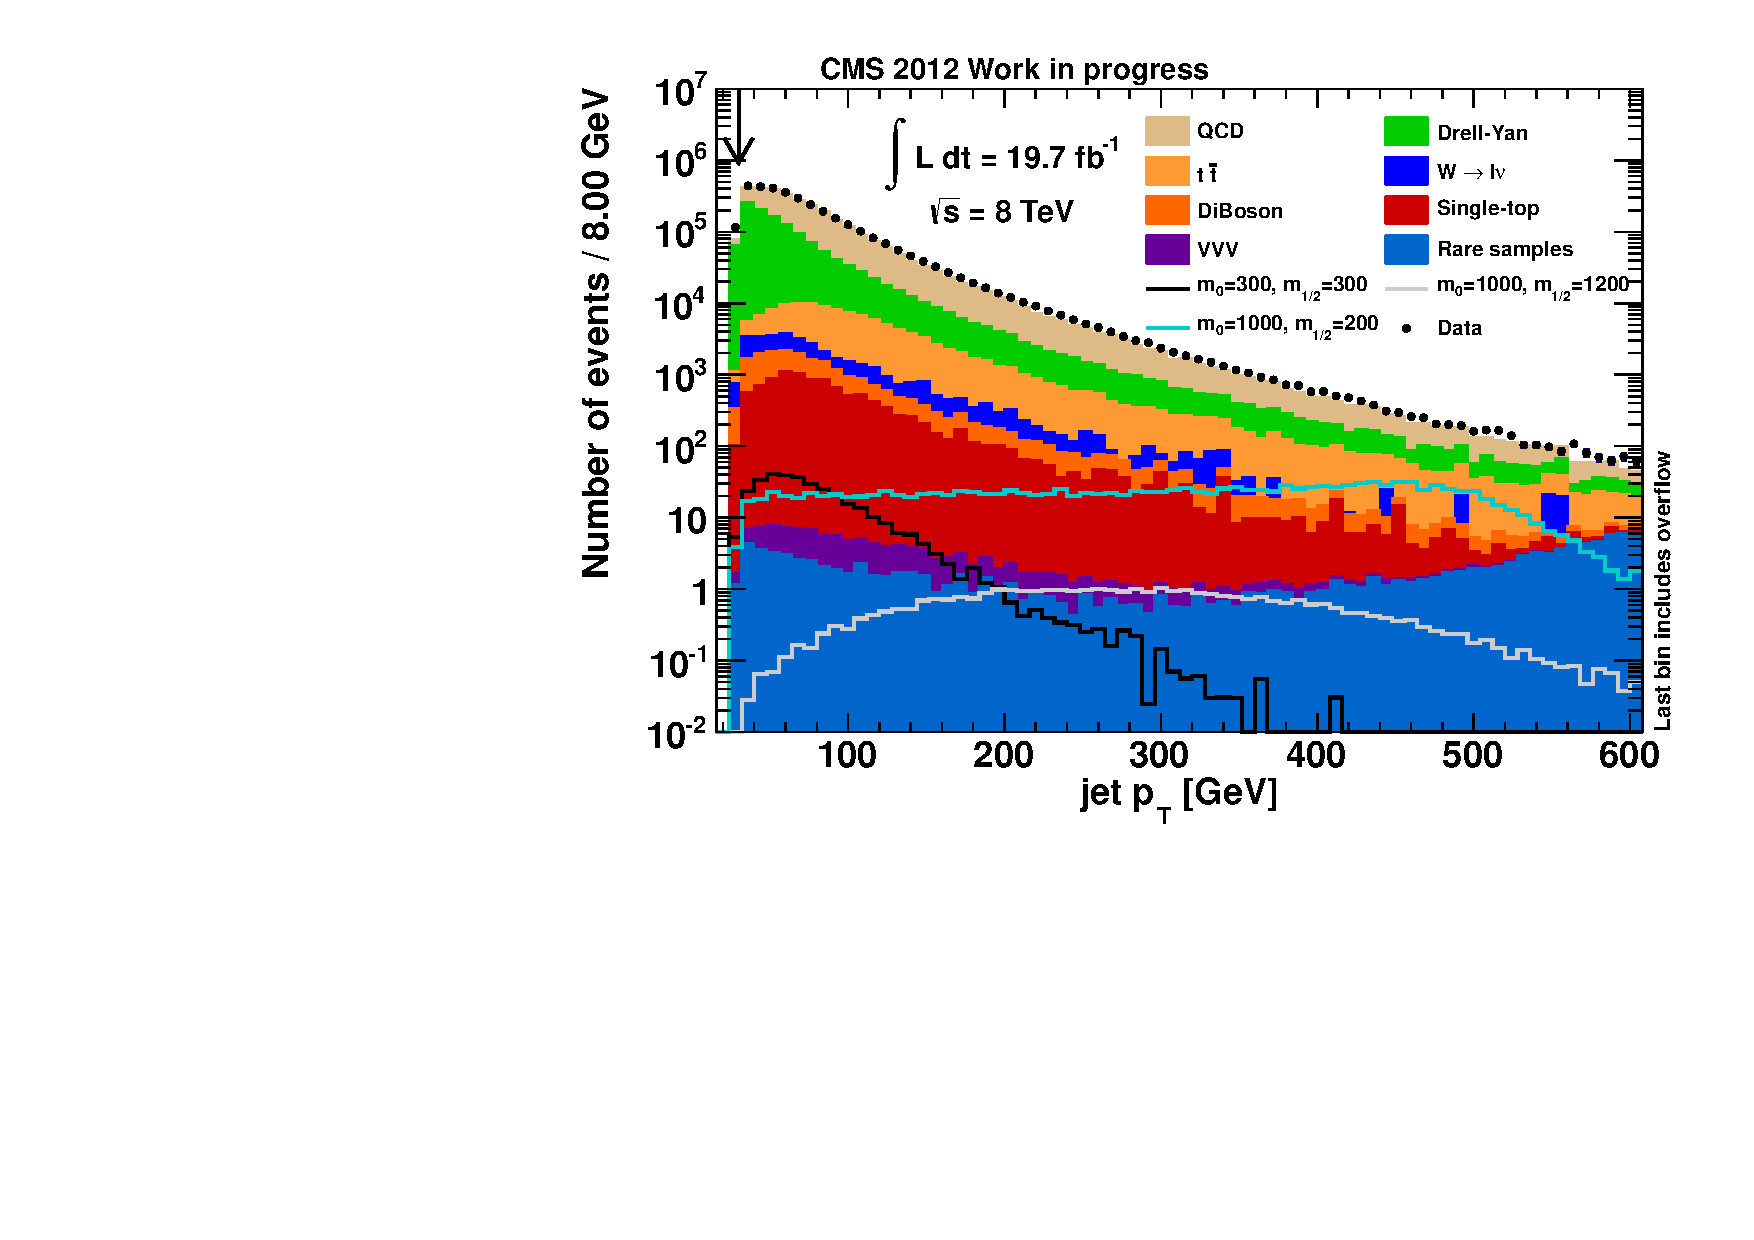
\includegraphics[width=\textwidth]{plots/jet_pt1.pdf}
    \caption{\label{fig:jetpt1}}
  \end{subfigure}
  \caption{Number of jets (\ref{fig:jetn}) and leading jet transverse momentum (\ref{fig:jetpt1}) at this stage of the analysis. The thresholds are at least two jets and $p_{\text{T}, j_1} > 30\,\text{GeV}$.}
  \label{fig:jetqualy}
\end{figure}

\noindent Although the thresholds also cut off a sizeable portion of the jet content for certain signal simulations, there is a sufficient number of events remaining. Thinking back to the selection efficiencies for the signal in section~\ref{sec:mcstudy}, this distribution displays how variable the impact of requirements can be.
 

\section{Muon Quality Criteria}
\label{sec:muonqualy}

To satisfy the signal signature and provide the candidates for further selection requirements, events containing exactly two ``good'' muons are selected. For this purpose the basic muon subset is refined through trigger-matching as well as isolation and impact parameters thresholds. It should be noted that the actual process of evaluating the events has been performed before the event cleaning. For the impact parameter, this was meant to prevent any bias. And in regards to the remaining parameters it was unavoidable, due to the structure of this analysis (see upcoming cha.~\ref{cha:datadrivenbg}).

Every \textit{event} examined at this stage is already required to pass the selected trigger (Sec.~\ref{sec:trigger}). Building upon that, the trigger-path for the \textit{muon} content of each event is also compared to the one of \verb+HLT_Mu17_TkMu8+ for every single particle. Only particles that fulfil this match are considered as candidates to ensures a minimum reconstruction quality and equal conditions throughout the entire subset. 

In addition to that, there are two different types of isolation criteria implemented. For the first one all calorimeter and tracker information are taken into account, thus naming the combined relative isolation $I_{\text{rel}}$. For its calculation, the following formula is suggested for all 2012 analyses.

\begin{equation}
  \label{eq:reliso}
  I_{\text{rel}} = \frac{ \sum p_{\text{T, charged had.}} + \max \left( 0,  \sum E_{\text{T, neutral had.}} + \sum E_{\text{T}, \gamma} - 0.5 \sum p_{\text{T, PU}} \right) }{ p_{\text{T}, \mu} }
\end{equation}

Each sum is determined by the particle flow algorithm. When adding them up, the $\Delta \beta$ corrections are applied to the neutral energy deposit. The corrections are based on the energies of charged particles not stemming from the primary vertex. These are determined by splitting particle flow candidates by whether or not they are considered to be pileup contributions. The factor of 0.5 has been determined from jets as an average of neutral to charged particles~\cite{muondbeta}.

The overall sum represents the energy/transverse momentum around the muon candidates in a cone with a radius of $R = 0.4$. Division by the particle's transverse momentum reduces the dependence on the energy of the interaction. With higher energies in the initial state, the absolute amount of energy carried by the all products is expected to rise as well. However, the relative distribution of said energy is expected to remain similar. With highly energetic muons and a relative isolation criterion, pileup contamination also becomes less of a problem for the same reason. Figure~\ref{fig:reliso} shows the combined relative isolation.

\begin{figure}[ht!]
  \centering
    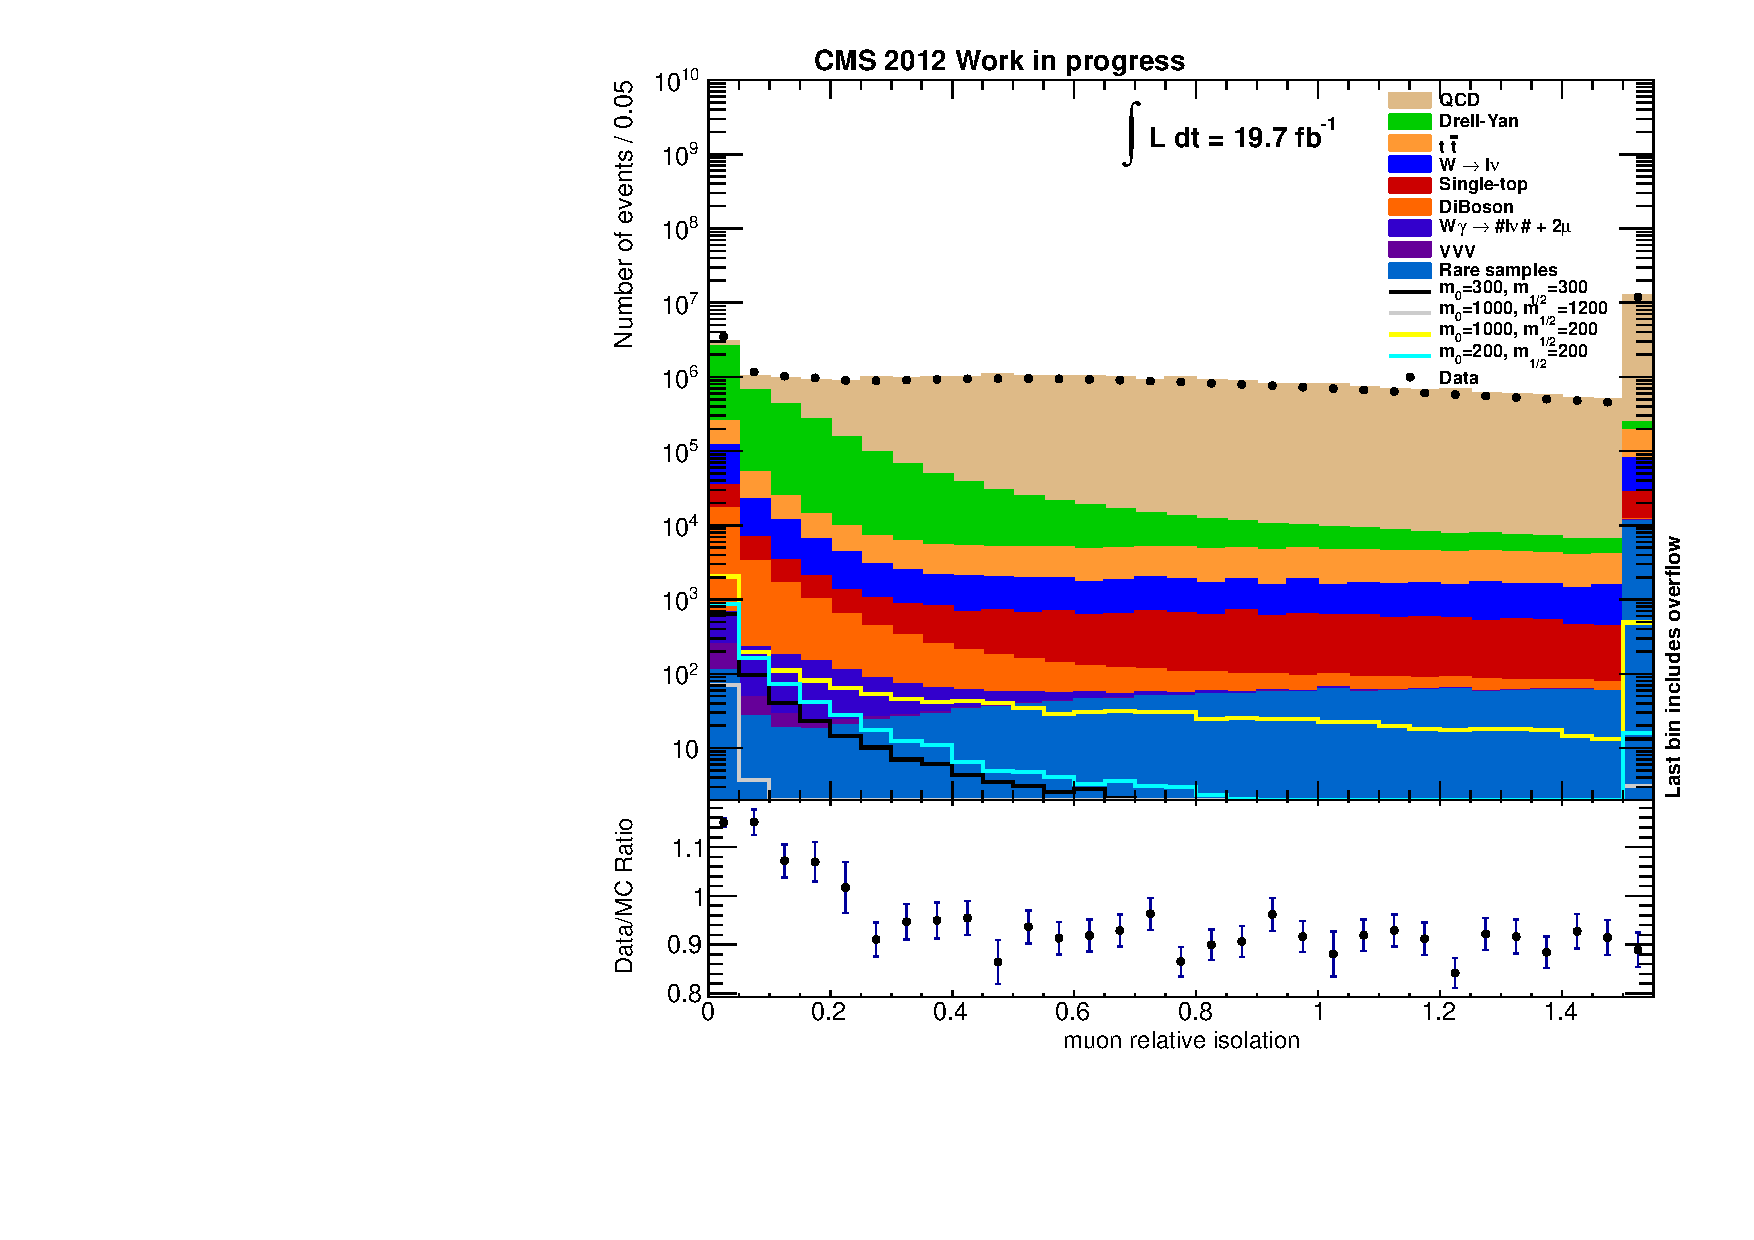
\includegraphics[width=0.7\textwidth]{plots/reliso.pdf}
  \caption{Combined relative isolation~\ref{eq:reliso} of muons. In the large overflow bin, the almost constant continuation of the distribution is contained. For this analysis, it is not of relevance. This histogram was generated before any selection of event.}
  \label{fig:reliso}
\end{figure}

\noindent For tight muons the recommended threshold value is $I_{\text{rel}} < 0.12$~\cite{muonpog}. As one can see, the majority of QCD events are rejected by this. Naturally, muons stemming from hadronic interactions are more likely to have fragments interfering with the isolation. Additionally, one can observe the signal simulations being affected differently. The softer decline for the high $m_0$ and low $m_{1/2}$ Monte Carlo will have a negative impact on the efficiency of selecting its events.

The second isolation criterion deals with the spatial distance $\Delta R$ between jets which pass the object selection and muons. It is required to be at least $0.4$ for each of the two muons candidates. Similarly to the combined relative isolation, this ensures that the muon has a reasonably clean trajectory to work with. Although in this case the emphasis is put on hadronic interferences instead of taking a combination of all of them.

Further restrictions are placed upon both the impact parameters. The muon POG suggests tightening the \textit{transverse} one to $d_{xy} < 0.2\,\text{mm}$. By reducing it by one order of magnitude, vertices  cosmic muons are suppressed more effectively. When comparing the \textit{longitudinal} impact parameters of both muons, the signal particles are expected to be very close to each other as the supersymmetric decays are effectively prompt. In figure~\ref{fig:deltadz}, the difference between the impact parameters of the two candidates is visualized.

\begin{figure}[ht!]
  \centering
    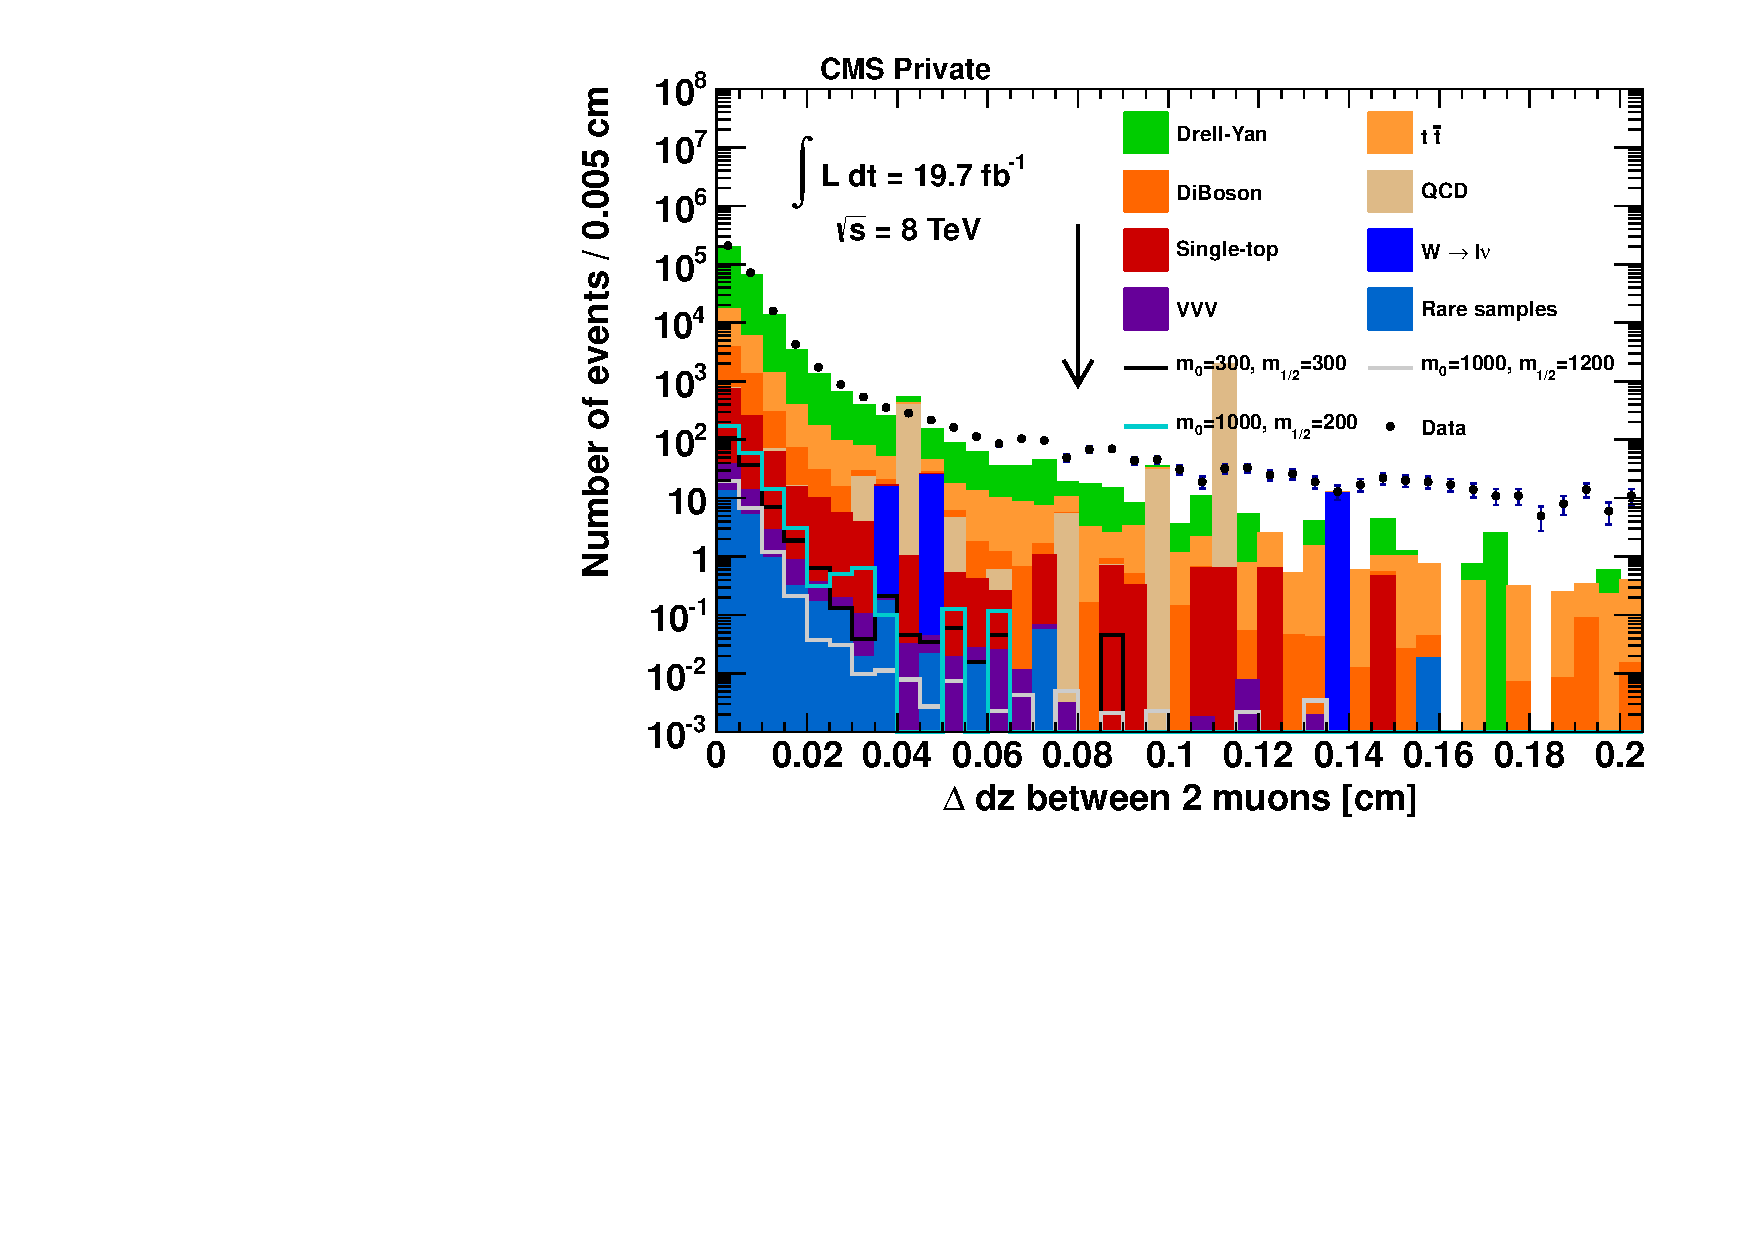
\includegraphics[width=0.6\textwidth]{plots/dz_mumu.pdf}
  \caption{Difference between the longitudinal impact parameter of the two muon candidates.}
  \label{fig:deltadz}
\end{figure}

\noindent Almost no signal events can be observed past $\Delta d_{z, \mu\mu} \leq 0.8\,\text{mm}$. Hence, the threshold is set to this value.

Only events with two muon candidates who suffice all listed requirements pass this stage of the selection.



\section{Scaling}
\label{sec:scaling}

After applying the muon quality criteria, the Drell-Yan background is the dominant one. However, upon closer inspection a discrepancy between data and simulation can be observed. To allow for better comparison between them, the scaling factor $f$ (Eq.~\eqref{eq:weight}) can be employed. It is a reasonable choice, since this background is not being used in the final distributions. Strictly speaking, this is not part of the event selection. Nevertheless the Drell-Yan background is most relevant at this stage, therefore the adjustment is performed here as well.

In figure~\ref{fig:m_mumu_zpeak_nodysf} and~\ref{fig:m_mumu_zpeak} the invariant mass of both selected muons is shown before and after the scaling, respectively.

\begin{figure}[htb!]
  \centering
  \begin{subfigure}[b]{0.495\textwidth}
    \centering
    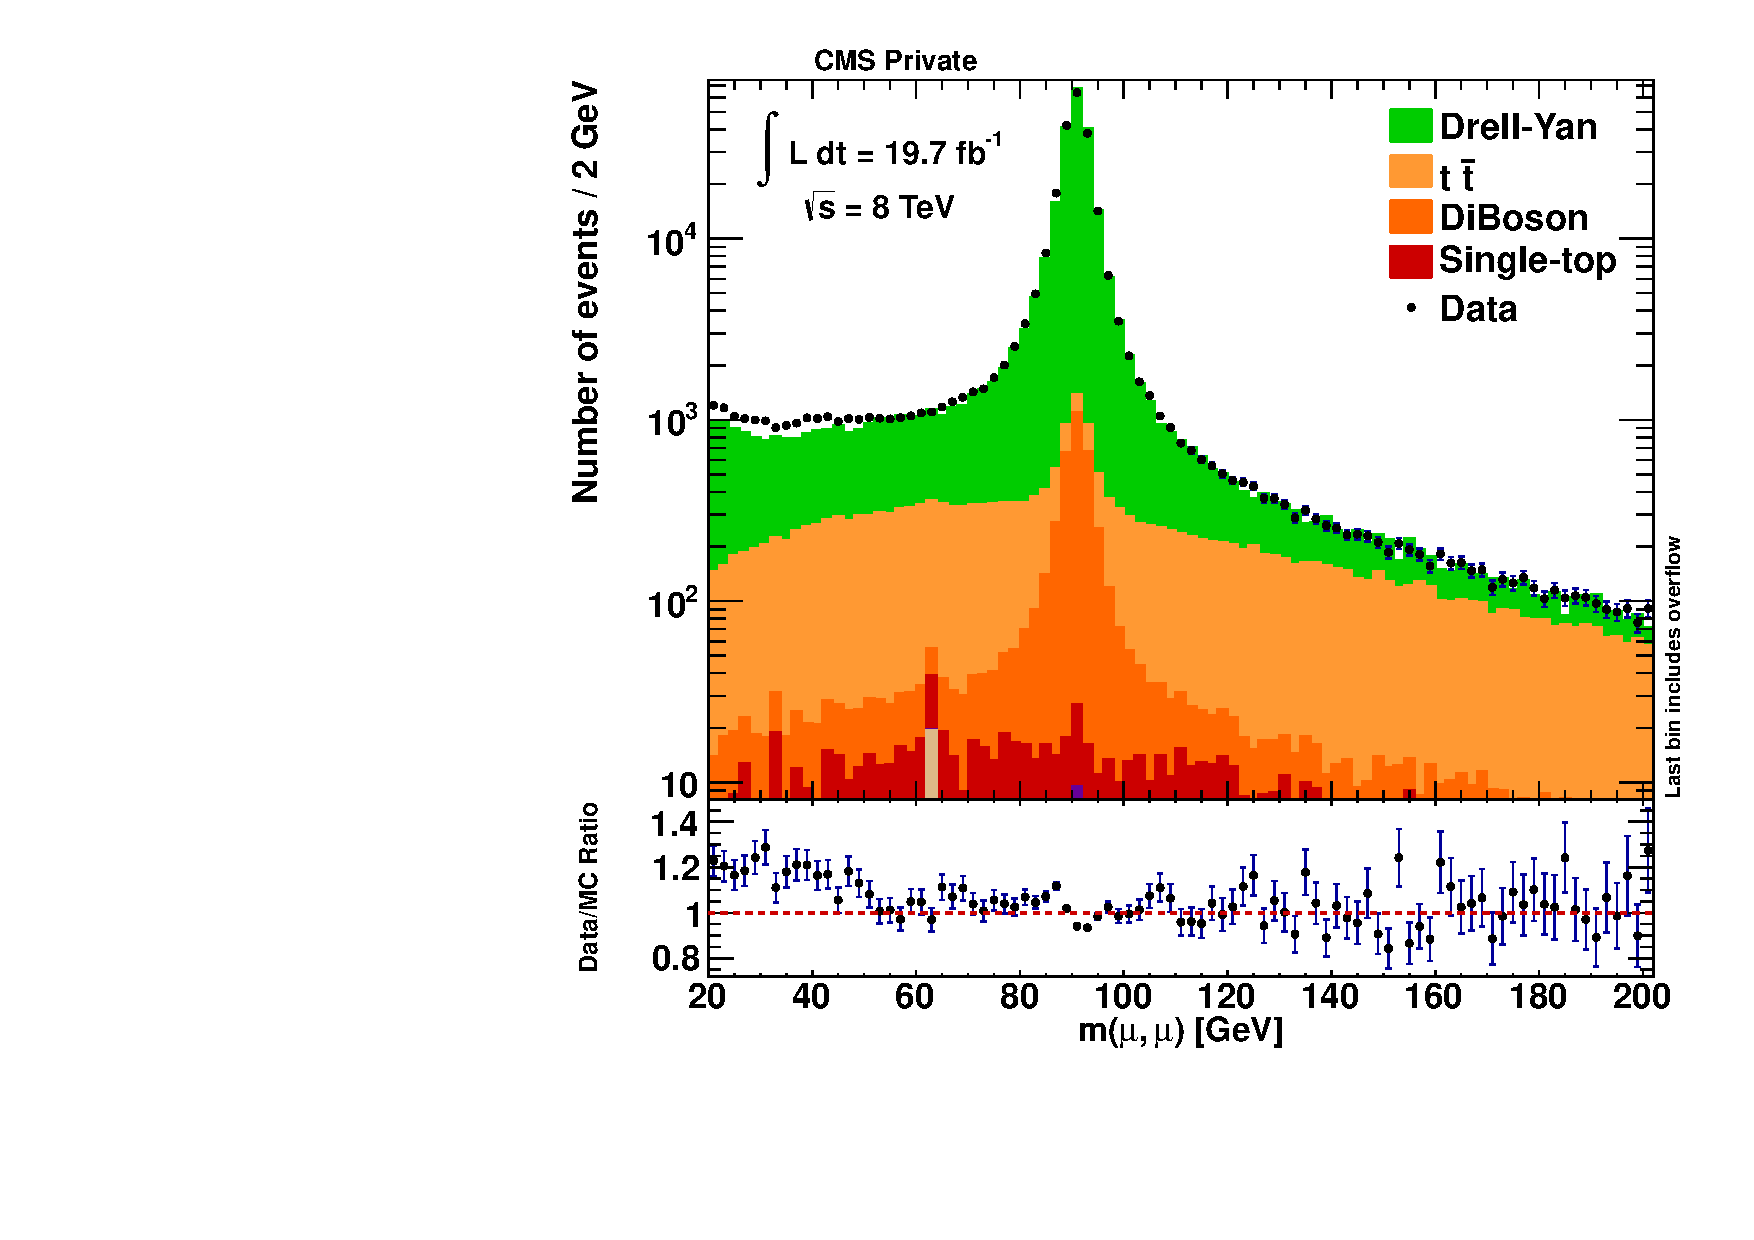
\includegraphics[width=\textwidth]{plots/m_mumu_zpeak_nodysf.pdf}
    \caption{\label{fig:m_mumu_zpeak_nodysf}}
  \end{subfigure}
  \begin{subfigure}[b]{0.495\textwidth}
    \centering
    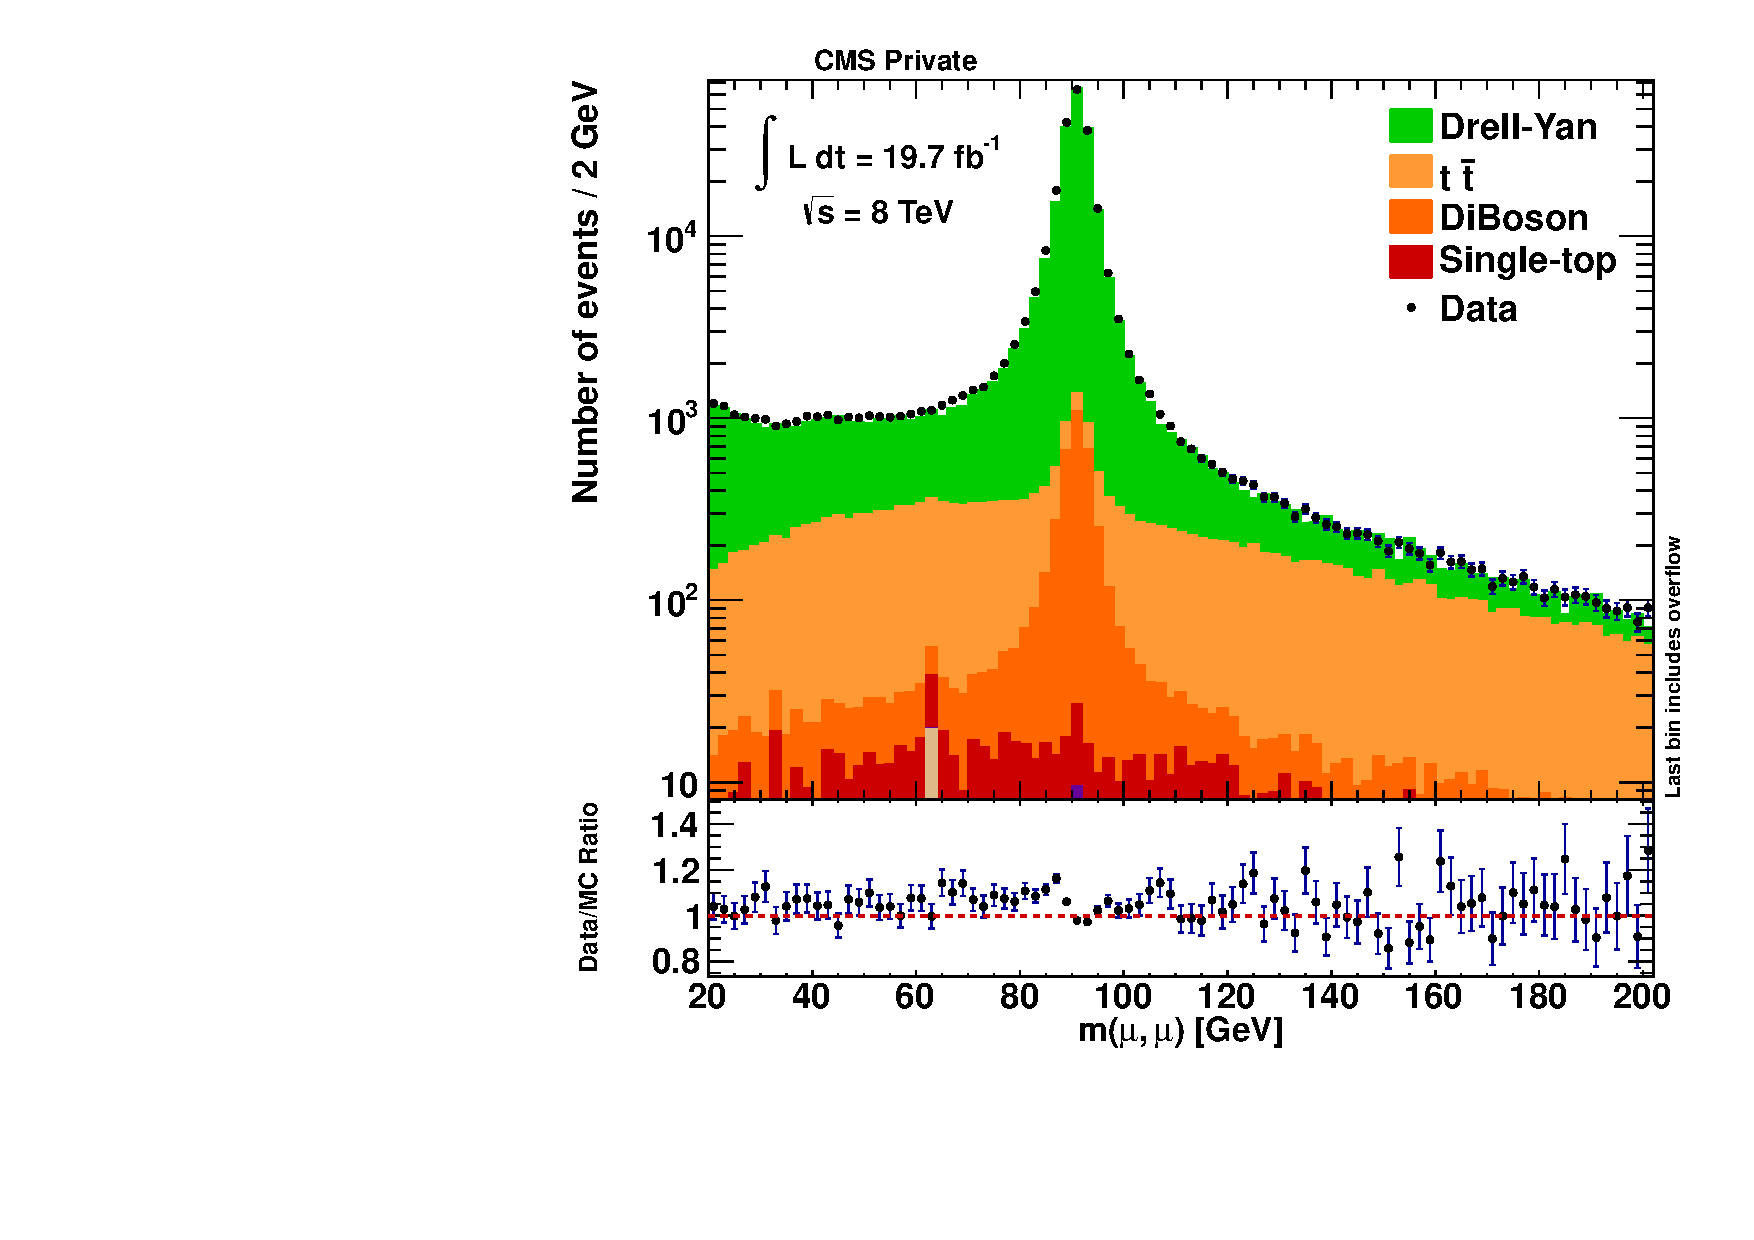
\includegraphics[width=\textwidth]{plots/m_mumu_zpeak.pdf}
    \caption{\label{fig:m_mumu_zpeak}}
  \end{subfigure}
  \caption{Invariant mass of the two selected muons. In histogram \ref{fig:m_mumu_zpeak_nodysf} the scaling factors for the Drell-Yan background are not applied, while in histogram \ref{fig:m_mumu_zpeak} they are.}
  \label{fig:dyscaling}
\end{figure}

\noindent Comparing both the entries centered around the $Z$-peak and especially the ones for lower invariant masses, one can observe a noticeable improvement. With the general shape of the data being well described, the assumption that the difference can be accounted for by a scale factor, holds true. 

The reasoning as to why one observes discrepancies is different for the two Drell-Yan samples. The first one ($10\,\text{GeV} < m_{ll} < 50\,\text{GeV}$) is only weighted with a leading order cross section. Thus a variation of $\mathcal{O}(10\pct)$ is easily within the realm of possibilities, as a next-to leading order calculation can have a similar impact. Since the second sample ($50\,\text{GeV} < m_{ll}$) is already weighted with a next-to-next-to leading order cross section, a significantly lower correction is expected. The overprediction in that region is attributed to the multi-jet background. The accuracy of simulating these is limited.

Determining the ratio between the integrals of data and simulation yields the scale factors. Both values $f_{10-50} = 1.23$ and $f_{50} = 0.96$ are within the expected range. They are applied throughout the entire analysis, including distributions preceding this section.


\section{Invariant Dimuon Mass}
\label{sec:m_mumu}

Due to the resonances in the low mass region of the muon pair, the background is increased in this region. This is shown in figure~\ref{fig:m_mumu_zpeak_zoom}, which is an enhancement of the low mass region of \ref{fig:m_mumu_zpeak}.

\begin{figure}[ht!]
  \centering
    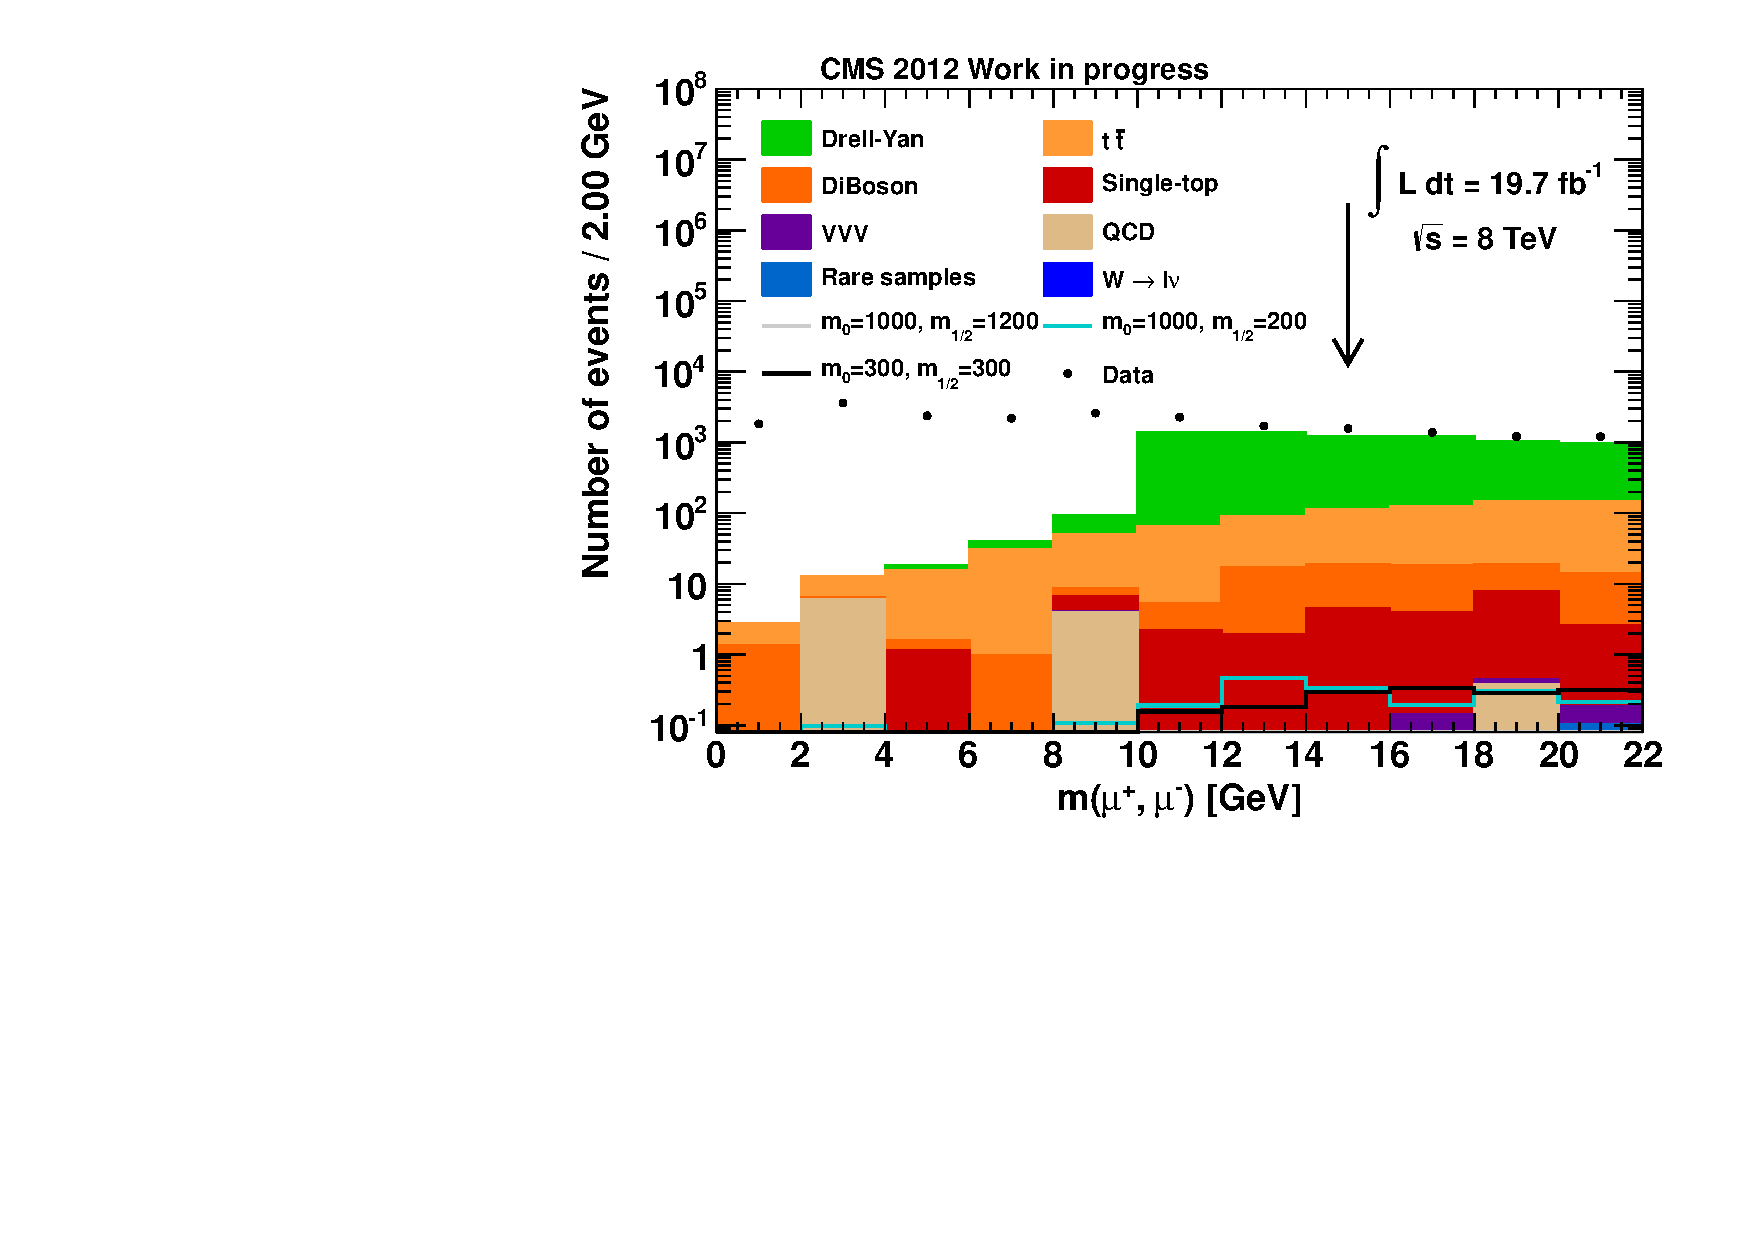
\includegraphics[width=0.7\textwidth]{plots/m_mumu_zpeak_zoom.pdf}
  \caption{Portion of the invariant dimuon mass distribution (Fig.~\ref{fig:m_mumu_zpeak}). The Drell-Yan Monte Carlo has only been generated down to $m_{ll} > 10\,\text{GeV}$.}
  \label{fig:m_mumu_zpeak_zoom}
\end{figure}

In the Drell-Yan Monte Carlo production these resonances were avoided, explaining its missing contribution in this region. Rejecting events with an invariant mass of the two selected muons below $15\,\text{GeV}$, is a safe choice to prevent any interference from resonances.


\section{Missing Transverse Energy}
\label{sec:met}

As discussed in chapter~\ref{cha:sig}, \textit{resonant} production of sleptons can lead to low amounts of missing transverse energy in the final state. In this analysis, MET has been computed using the particle flow algorithm. The corresponding histogram is given in figure~\ref{fig:pfmet}.

\begin{figure}[ht!]
  \centering
    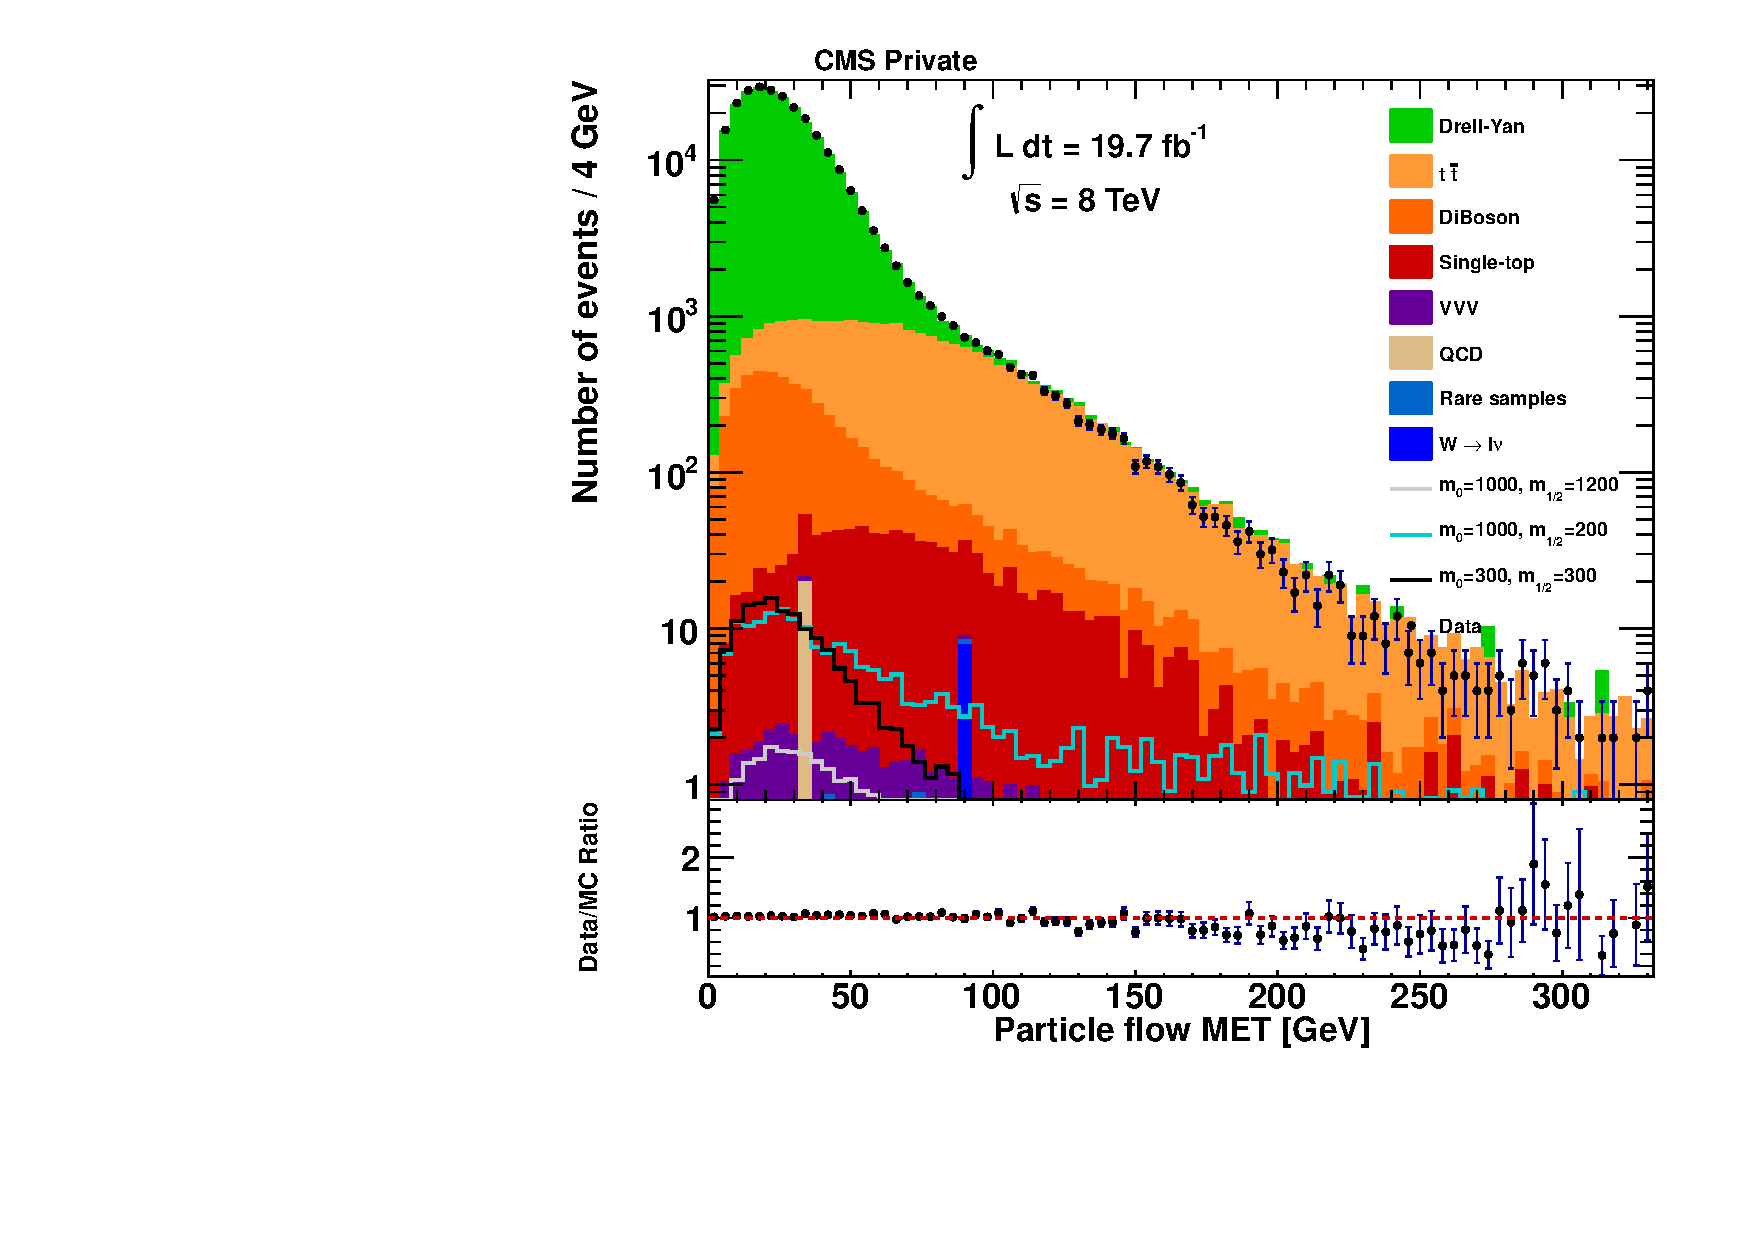
\includegraphics[width=0.7\textwidth]{plots/pfmet.pdf}
  \caption{Particle Flow missing transverse energy.}
  \label{fig:pfmet}
\end{figure}

The distribution shows very good agreement up until roughly $200\,\text{GeV}$. Here one can see a slight systematic overprediction. The $t\bar{t}$ sample which dominates this region, has been generated with \textsc{Powheg}. Due to that additional jets pose more of a challenge. Combined with the higher jet multiplicity towards higher energies, the discrepancy is comprehensible. One can also see that the majority of the signal contribution is concentrated in the region with very little MET. Once again, the shape of the signal varies between the different regions of the phase space. Compared to the other simulations, the selection efficiency for the high $m_0$, low $m_{1/2}$ point suffers a lot due to the softer decline. To optimize the signal to background ratio for the majority of SUSY parameter configurations, the threshold is set at $E^{\text{miss}}_{\text{T}} < 50\,\text{GeV}$.

To be able to judge the quality of the last steps of the event selection without consulting the final distributions, control regions are introduced. The orthogonal sample is generated by inverting the missing transverse energy requirement. Demanding values larger than $50\,\text{GeV}$, is the first step for every control region. They are subsequently divided by their corresponding requirement passing or rejecting events.


\section{Jets From b-Quarks}
\label{sec:bjets}

The signal signature (Cha.~\ref{cha:sig}) only includes jets from the first generation of quarks. With the top quark backgrounds being amongst the most dominant ones, a sizeable amount of jets will stem from bottom quarks. To reduce their contribution in the final distributions, the combined secondary vertex algorithm (\textbf{CSV})~\cite{csvbtag} is used. 

This very sophisticated algorithm combines a multitude of parameters to distinguish $b$-jets from non-$b$-jets. Its basis is the reconstruction of secondary vertices produced in the weak decay of bottom quarks. For that purpose the Trimmed Kalman Vertex Finder~\cite{kalmanvtx} is employed. Starting off with all tracks assigned to a jet, it isolates rogue ones. These are then used to reconstruct new vertices, which are sorted into three categories. For the first one, the candidates have to suffice four criteria.

\begin{itemize}
\item The $x$-$y$-distance $l_{\text{T}}$ between primary and secondary vertex has to be larger than $100\,\mu\text{m}$ but within $2.5\,\text{cm}$.
\item The significance of said distance $\frac{l_{\text{T}}}{\sigma_{l_{\text{T}}}}$ has to be larger than $3$
\item The invariant mass of all charged particles must not be larger than $6.5\,\text{GeV}$.
\item If there are two tracks with opposite charges, their mass must not be within $50\,\text{MeV}$ of the $K^0_S$ mass.
\end{itemize}

\noindent If all requirements are met, the candidate is considered a reconstructed secondary vertex. Should they not be met, but there are still at least two tracks with the specified significance higher than 2, a ``pseudo-vertex'' is created. This is the second category. If neither situation applies to the jet, it is placed in the third one.

Based on which category a jet belongs to, the criteria are tightened and/or expanded upon. Relevant variables for the identification of $b$-jets are the following ones.

\begin{itemize}
\item The invariant mass of all charged particles belonging to a secondary vertex can be compared to the one of charm quarks. If it is significantly higher, this can be used to veto against $c$-quarks.
\item A high multiplicity of tracks is characteristic to $b$-jets, even compared to charm hadrons.
\item Since bottom quarks have a comparatively long flight time, the significance $\frac{l_{\text{T}}}{\sigma_{l_{\text{T}}}}$ can be examined further.
\item The energy fraction of all charged particles of the secondary vertex as well as the one of the entire jet can be compared to the hard fragmentation function of quarks.
\item Due to the large mass of a bottom quark, the produced particles are on average more collimated than e.g. $c$-quarks. Therefore the pseudorapidity can be used.
\item Sorting the tracks by their impact parameter significance and determining their invariant mass can help against $c$-quarks as well. The first track exceeding the charm's specific threshold $1.5\,\text{GeV}$ can be used to split them into two categories.
\end{itemize}

\noindent While all of them can be incorporated for the first category of vertices, the significances have to be excluded for the second one. The reason behind this is the lack of a geometrical fit for this type of vertex. For the third category no additional variables are used.

To derive a single value $d$ for discrimination, all variables are combined into a likelihood function $\mathcal{L}$. Since light ($u$, $d$, $s$, $c$) and charm quarks lead to different parameter distributions, they are handled separately. $d$ is then given by

\begin{equation}
  \label{eq:btagdiscriminator}
  d = f_{\text{BG}}(c) \cdot \frac{\mathcal{L}^b}{\mathcal{L}^b + \mathcal{L}^c} + f_{\text{BG}}(q) \cdot \frac{\mathcal{L}^b}{\mathcal{L}^b + \mathcal{L}^q} \quad \text{with} \quad \mathcal{L}^{b, c, q} = \mathcal{L}^{b, c, q} (\alpha, x_i)
\end{equation}

\noindent The $\mathcal{L}$ are a function of the vertex category denoted by $\alpha$ and the $x_i$, which denote the variables. Both $f_{\text{BG}}(c)$ and $f_{\text{BG}}(q)$ are the expected probabilities for light and charm jets to contain $b$ and $c$ quarks, respectively.

\begin{figure}[htb!]
  \centering
  \begin{subfigure}[b]{0.495\textwidth}
    \centering
    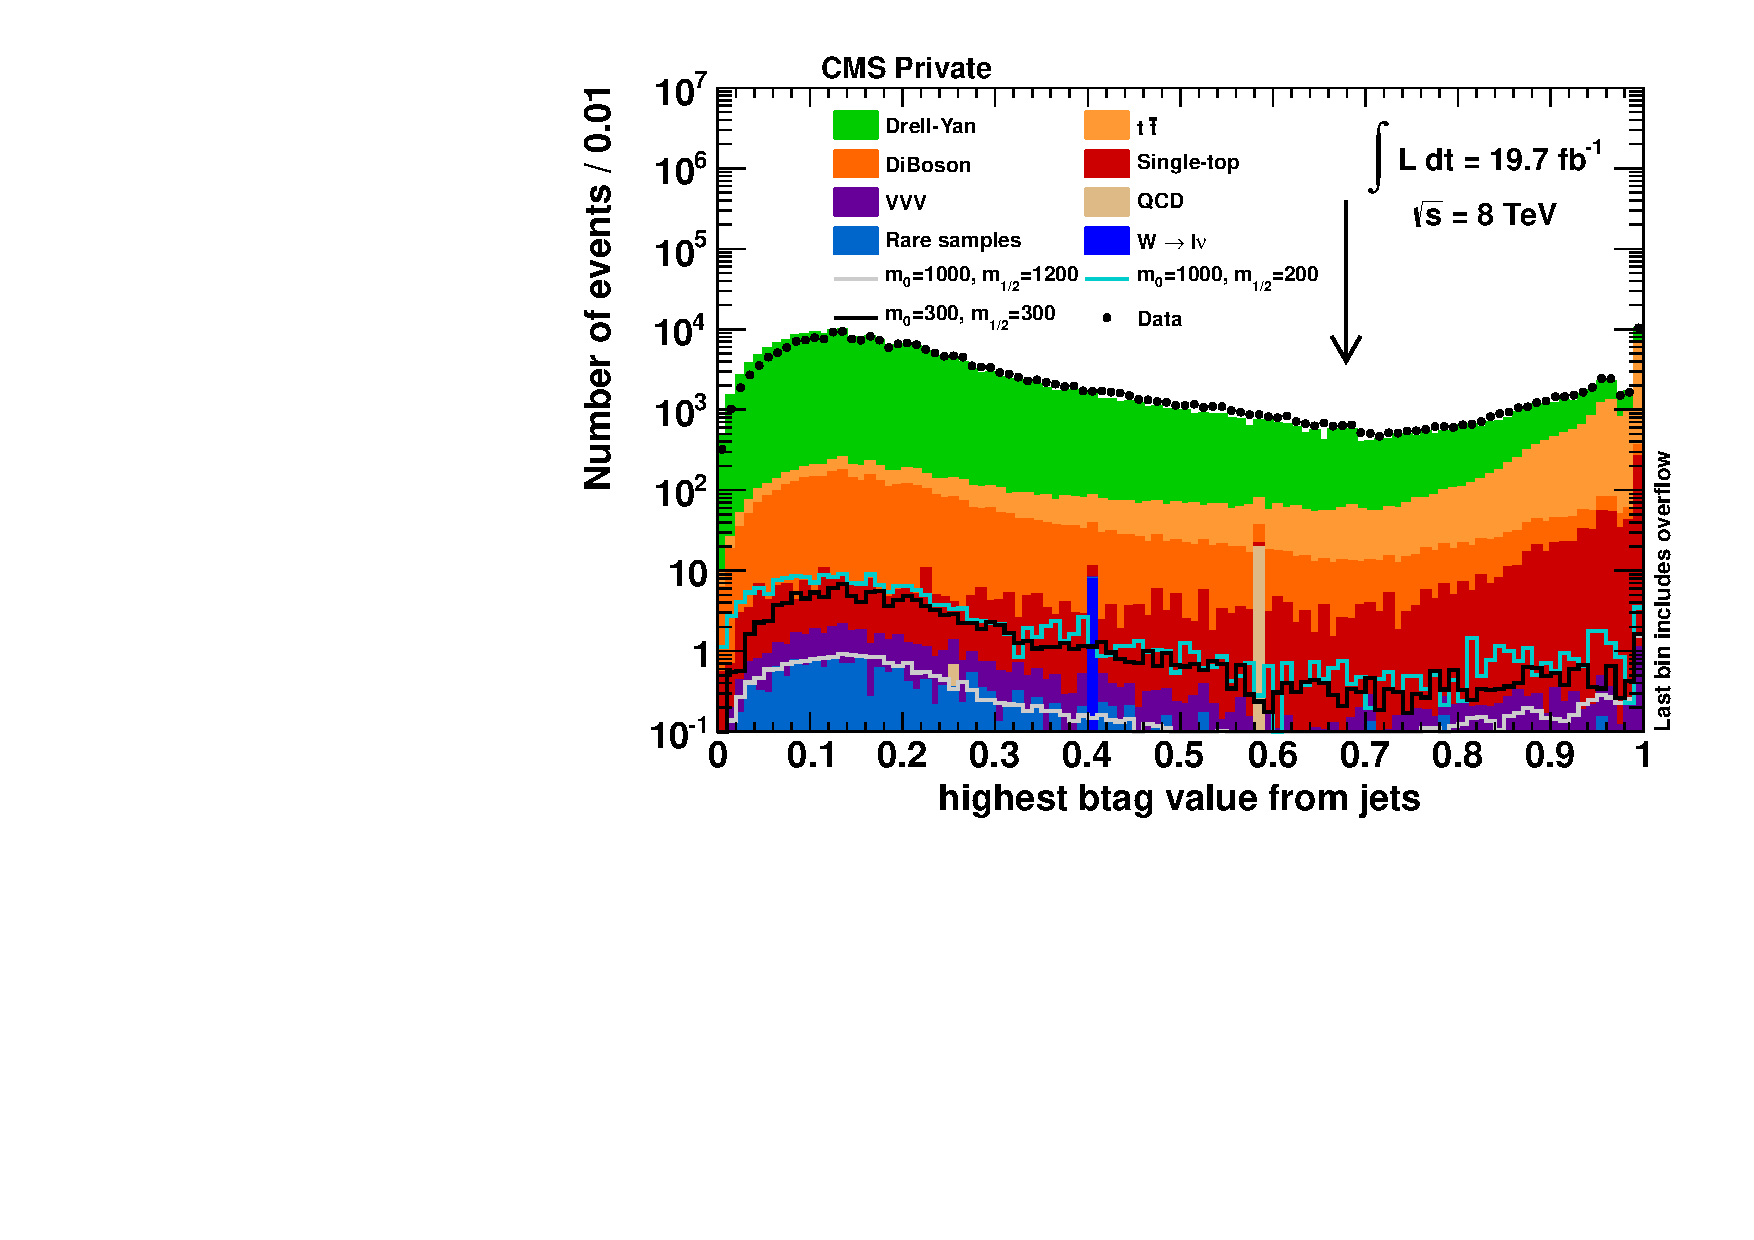
\includegraphics[width=\textwidth]{plots/1st_btag.pdf}
    \caption{\label{fig:1st_btag}}
  \end{subfigure}
  \begin{subfigure}[b]{0.495\textwidth}
    \centering
    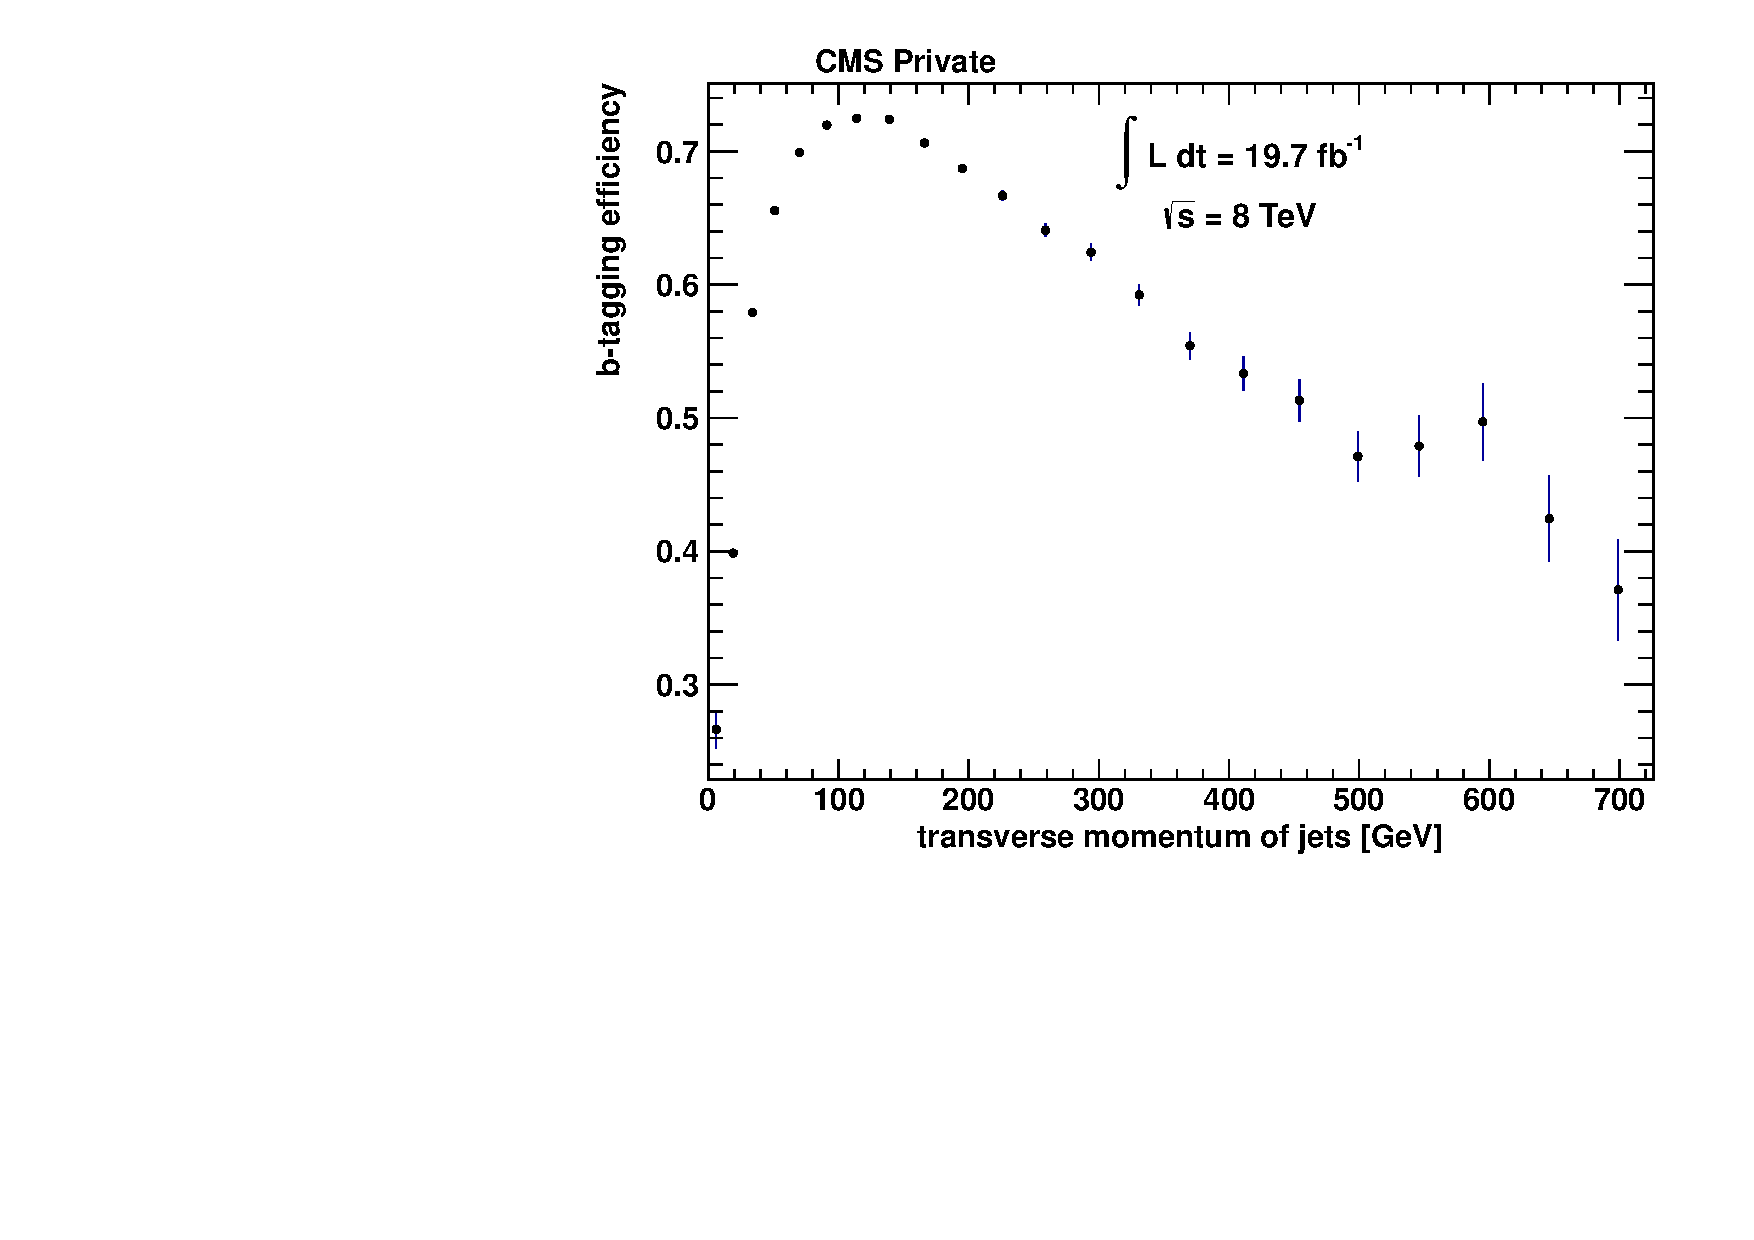
\includegraphics[width=\textwidth]{plots/b_proj.pdf}
    \caption{\label{fig:b_proj}}
  \end{subfigure}
  \caption{Highest $b$-tag discriminator of an event \ref{fig:1st_btag} and $p_{\text{T}}$-projection of the Monte Carlo $b$-tagging efficiency \ref{fig:b_proj}.}
  \label{fig:btag}
\end{figure}

The medium working point for the CSV (\textbf{CSVM}) has been chosen for this analysis. Its suggested dicriminator value is $d > 0.679$~\cite{btagworkp}. To judge its performance, one can consult the distribution of the highest $b$-tag discriminator in every event shown in figure~\ref{fig:1st_btag}. One can see the majority of the top pair background being cut off by the chosen threshold. As expected, the signal simulation has its lowest contribution in this region as well. It is quite apparent that there are inefficiencies of the algorithm, especially towards the lower discriminator values. They are being accounted for by adjusting the $b$-tag status of a fraction of all jets\footnote{Once again $b$, $c$ and light jets are treated separately.}~\cite{btageff}. Depending on whether one needs to upgrade a non-tagged or downgrade a tagged object, a different formula for determining said fraction $f$ has to be used.

\begin{align}
  \label{eq:btagsf}
  f = 1 - \text{SF} \quad & \text{for} \quad \text{SF} < 1\:(\text{downgrade}) \\
  f = \frac{1 - \text{SF}}{1- 1/\varepsilon_{\text{MC}}} \quad & \text{for} \quad \text{SF} > 1\:(\text{upgrade})
\end{align}

\noindent Here, $\varepsilon_{\text{MC}}$ denotes the efficiency of the algorithm accurately selecting bottom quark jets in the Monte Carlo simulation. The scale factors $SF$ are defined by dividing the same efficiency measured in data by Monte Carlo one: $\text{SF} = \varepsilon_{\text{DATA}} / \varepsilon_{\text{MC}}$.

While the scale factors are provided as $p_{\text{T}}$ and $\eta$ dependent functions on the $b$-tagging TWiki~\cite{btagtwiki}, the Monte Carlo efficiency has to determined individually for each analysis. This is due to its dependence on the relevant background samples. Calculating the ratio of jets tagged by the CSVM algorithm to their true flavour yields $\varepsilon_{\text{MC}}$. The flavour can be retrieved by the jet flavour tool~\cite{jetflavtool}. It uses Monte Carlo generator information to determine the origin of a jet. Counting the numbers of tags for the denominator and true $b$-jets for the enumerator with respect to their $p_{\text{T}}$ and $\eta$ is done after adjusting the jet energy resolution of the Monte Carlo samples. The efficiency is only estimated using the $t\bar{t}$ background as it is the most relevant one for this requirement. Figure~\ref{fig:b_proj} shows the $p_{\text{T}}$-projection of the Monte Carlo efficiency map. For increasing $\eta$ values the shape remains the same, with slightly decreasing efficiencies ($\mathcal{O}(1\pct)$) for all bins. Towards higher energies, the number of entries and therefore the statistical uncertainty does not allow for reasonable estimate of the efficiency anymore. The value of the last bin is used for any jet exceeding the energy maximum. To get a model prediction, rather than being influenced by a few single bins with abnormal values, the \textsc{ROOT} smoothing algorithm has been employed. It estimates the contents of a bin by taking its neighbouring ones into account.

\begin{figure}[htb!]
  \centering
  \begin{subfigure}[b]{0.495\textwidth}
    \centering
    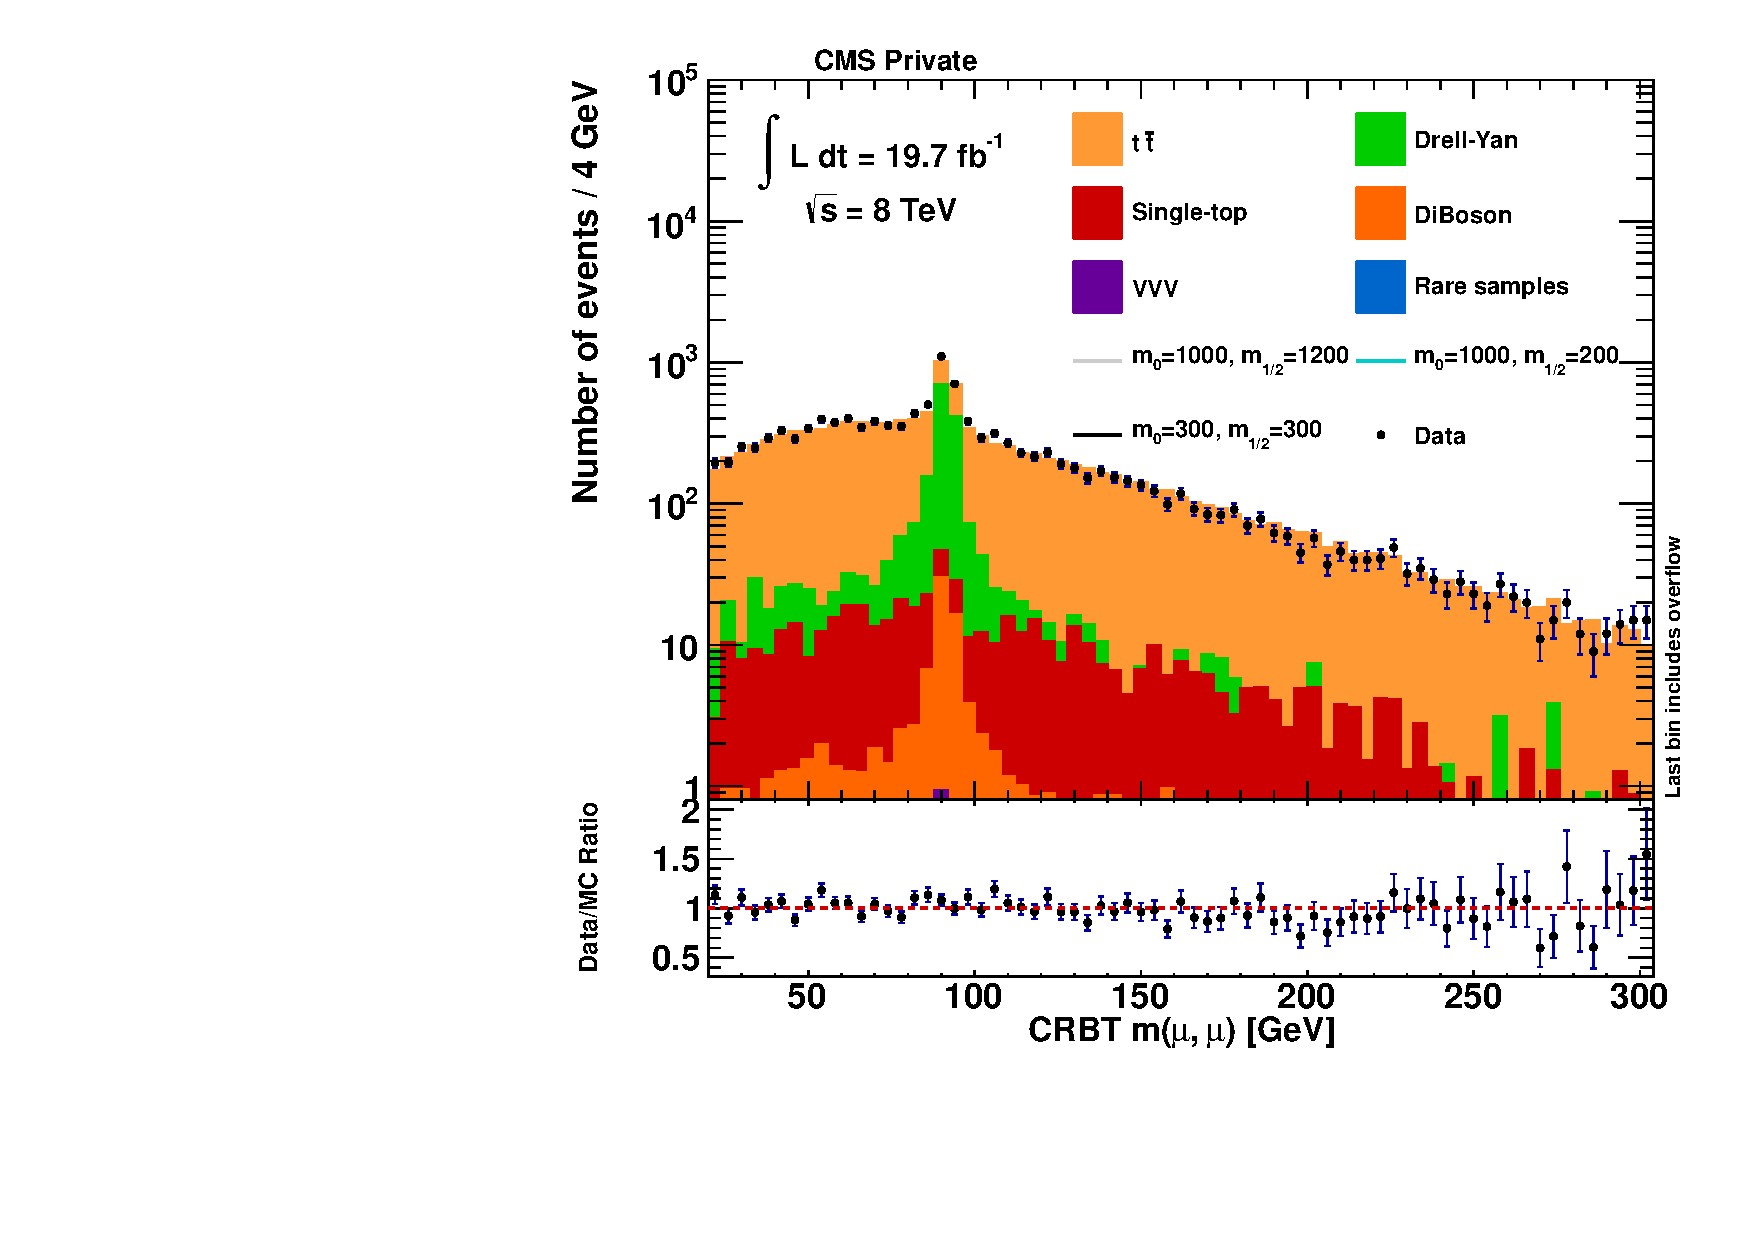
\includegraphics[width=\textwidth]{plots/crbt.pdf}
    \caption{\label{fig:crbt}}
  \end{subfigure}
  \begin{subfigure}[b]{0.495\textwidth}
    \centering
    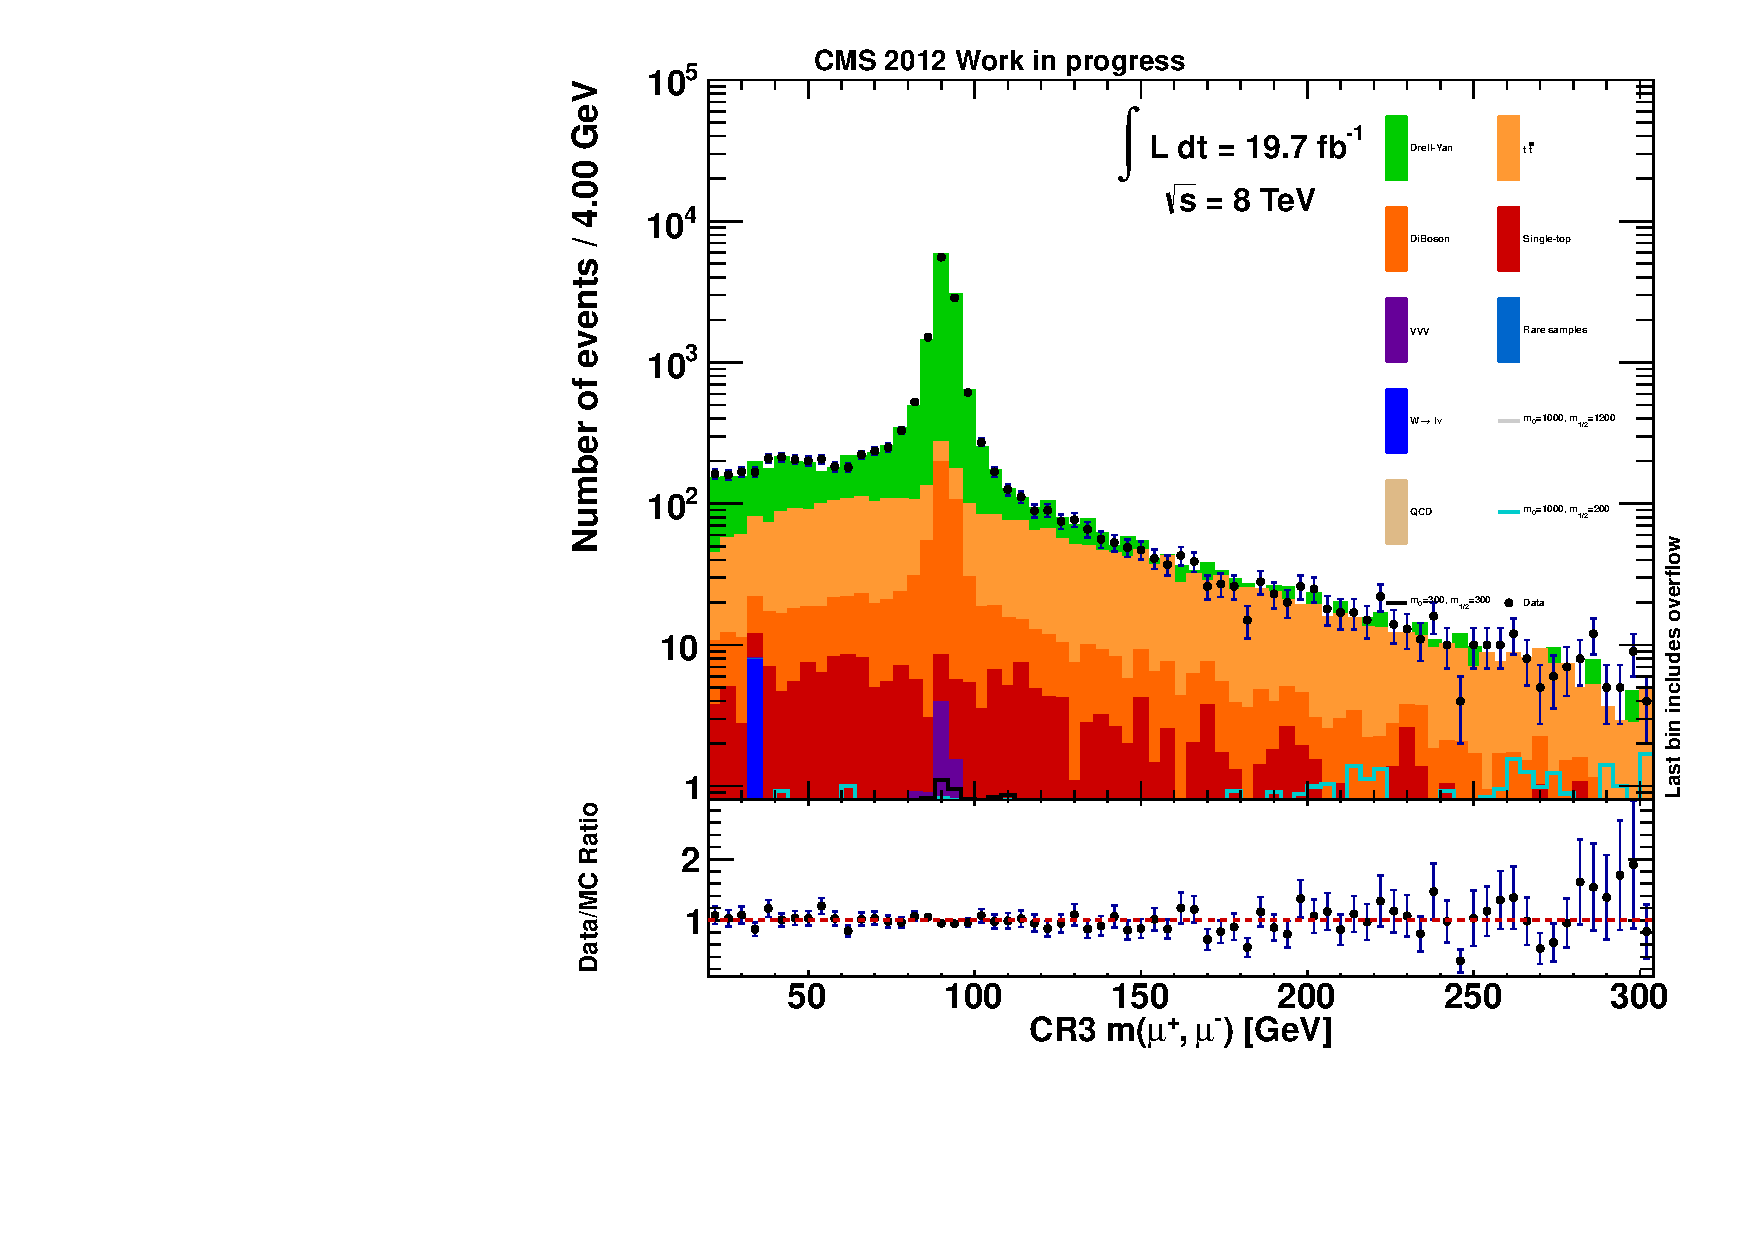
\includegraphics[width=\textwidth]{plots/crbv.pdf}
    \caption{\label{fig:crbv}}
  \end{subfigure}
  \caption{Control regions (MET $> 50\,\text{GeV}$) that display the effect of the $b$-tagging algorithm. On the left the $b$-tagged events \ref{fig:crbt} and on the right $b$-jet vetoed events \ref{fig:crbv} are shown.}
  \label{fig:crbtagging}
\end{figure}

With a set algorithm to tag $b$-jets, the control regions can be inspected to judge its performance. Figure~\ref{fig:crbt} shows the control region with events that are tagged as $b$-jets (\textbf{CRBT}) and will therefore be rejected. Complementary to that, figure~\ref{fig:crbv} displays the remainder of events after vetoing against $b$-jets (\textbf{CRBV}). Both distributions show good agreement between data and simulation. Combined with the majority of the rejected entries being from the top pair background, this entire method successfully reduces the bottom quark jet contribution in the final state.


\section{Same Sign Charge Muons}
\label{sec:sscmuons}

At this stage of the analysis, there is still \textit{at least} one order of magnitude between data and a potential signal. As discussed in the chapter regarding the signature (Cha.~\ref{cha:sig}), the charge of both prompt muons can be the same. Most of the background Monte Carlo cannot lead to the same condition in the final state. As a result, this requirement is able to improve the signal to background ratio significantly.

\begin{figure}[htb!]
  \centering
  \begin{subfigure}[b]{0.495\textwidth}
    \centering
    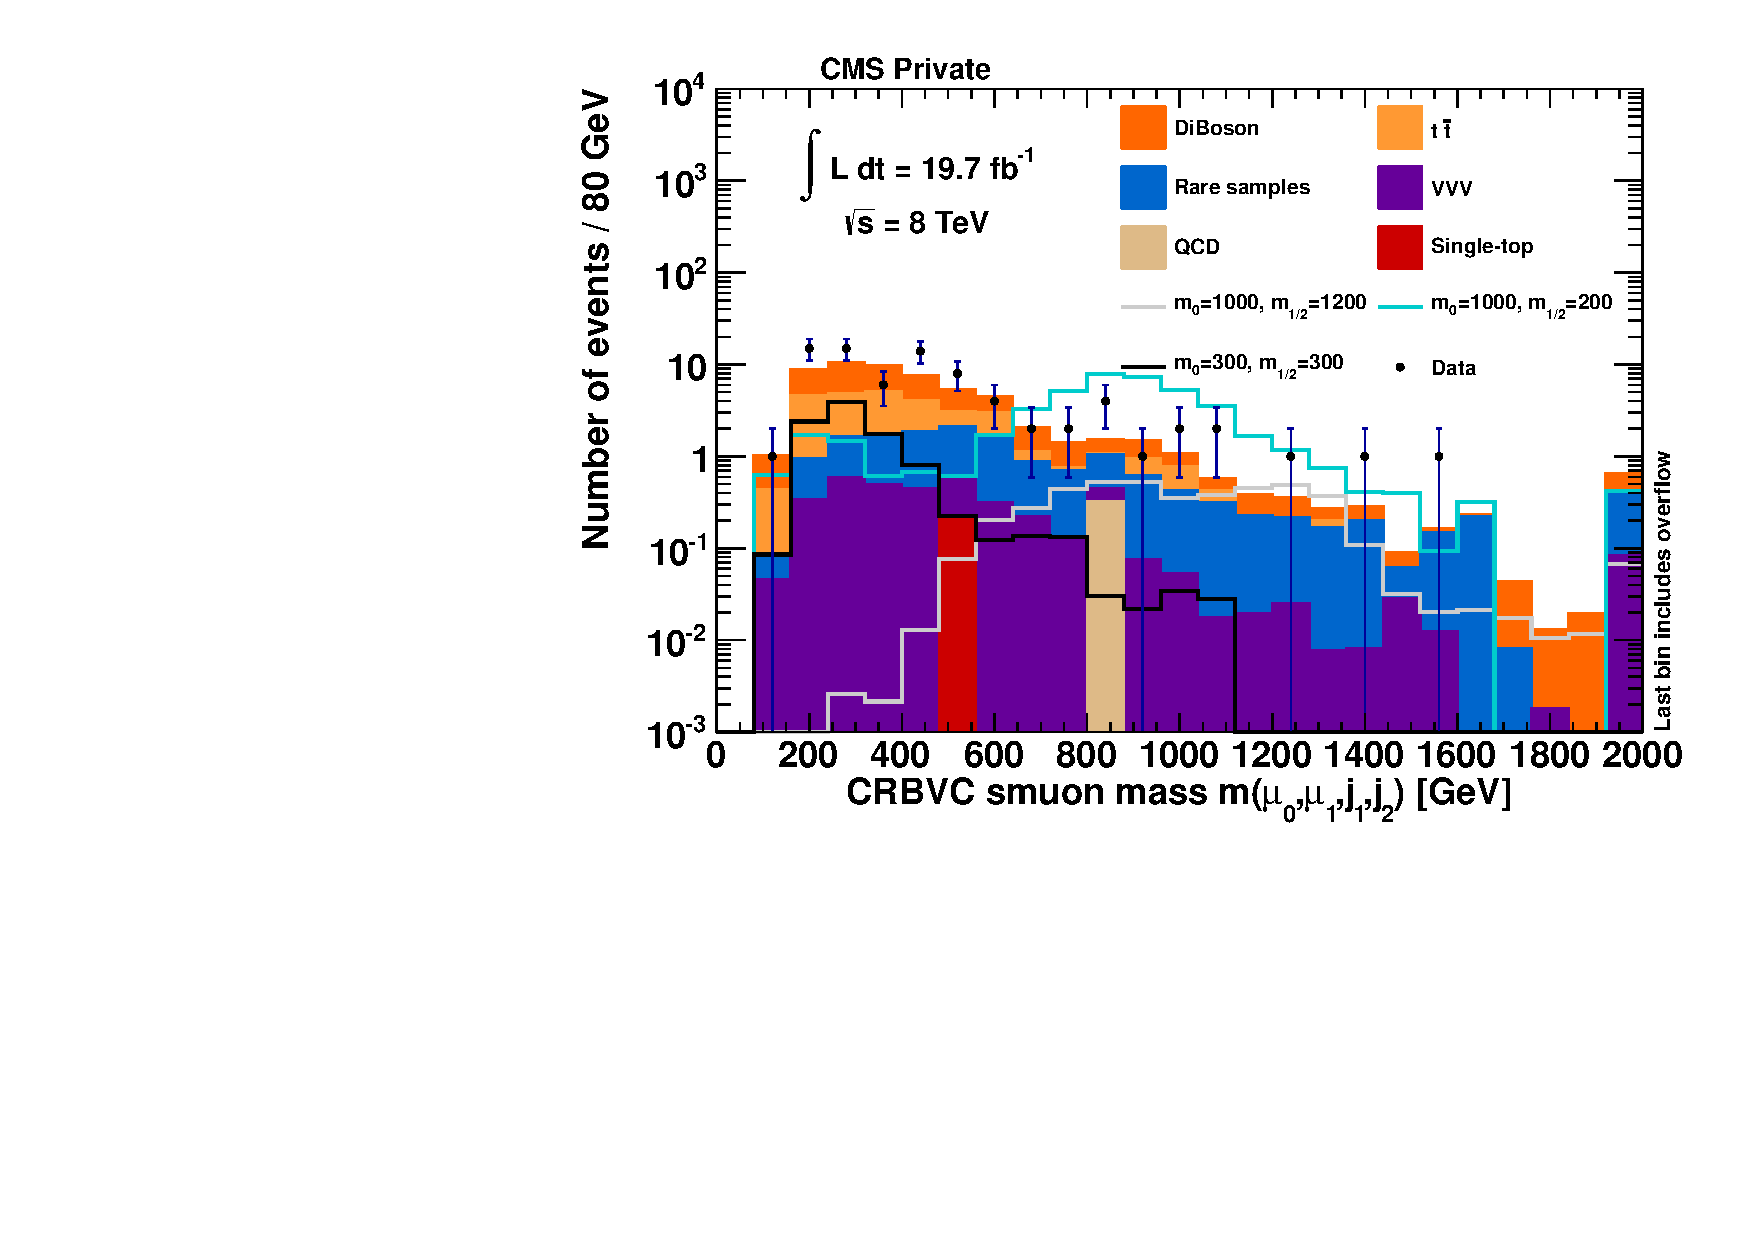
\includegraphics[width=\textwidth]{plots/CR6_m_smuon_nofakes.pdf}
    \caption{\label{fig:CRBVC_m_smuon_nofakes}}
  \end{subfigure}
  \begin{subfigure}[b]{0.495\textwidth}
    \centering
    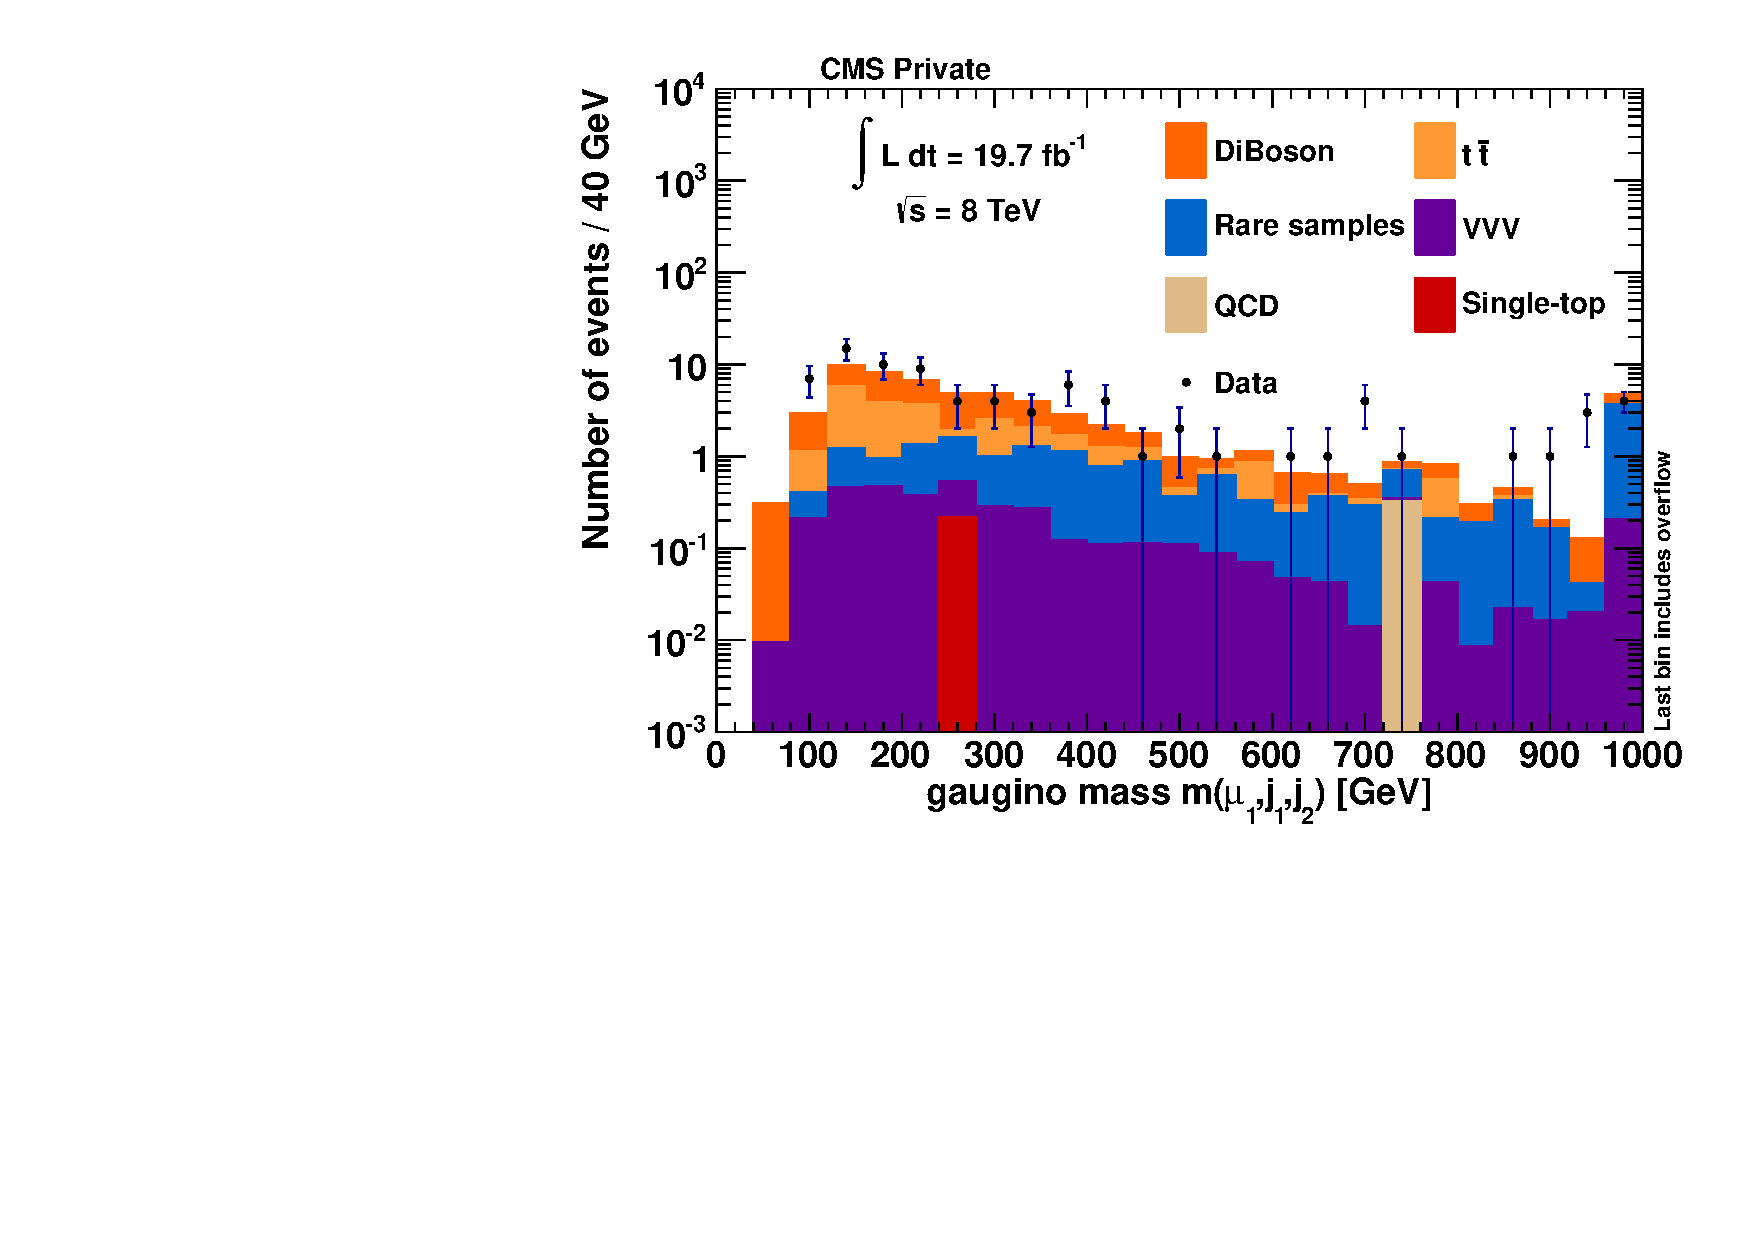
\includegraphics[width=\textwidth]{plots/CR6_m_gaugino_nofakes.pdf}
    \caption{\label{fig:CRBVC_m_gaugino_nofakes}}
  \end{subfigure}

  \caption{Mass of the gaugino \ref{fig:CRBVC_m_gaugino_nofakes} and mass of the smuon \ref{fig:CRBVC_m_smuon_nofakes} from the same sign charge control region. The gaugino mass is the invariant mass of both jets and the sub-leading muon, while the smuon mass includes the leading muon as well. Both distributions will be expanded upon in the following chapter.}
  \label{fig:ssccr_nofakes}
\end{figure}

The corresponding control region adds the charge restriction (\textbf{CRBVC}) to the previously defined CRBV. When examining the distributions of CRBVC (Fig~\ref{fig:ssccr_nofakes}), one does see the drastic reduction of the background. However, the dominant backgrounds are not amongst those, that are able to provide two prompt same sign charge muons from the same vertex. Additionally, data and simulation appear to be not in agreement throughout the entire mass spectrum. In combination, this suggests that the background is not described accurately. One effect that contributes significantly to this phenomena will be discussed in the upcoming chapter.


%%% Local Variables: 
%%% mode: latex
%%% TeX-master: "document"
%%% End: 
